\chapter{Stress minimisation}
\label{chap:stress}
\begin{figure}
  \centering
  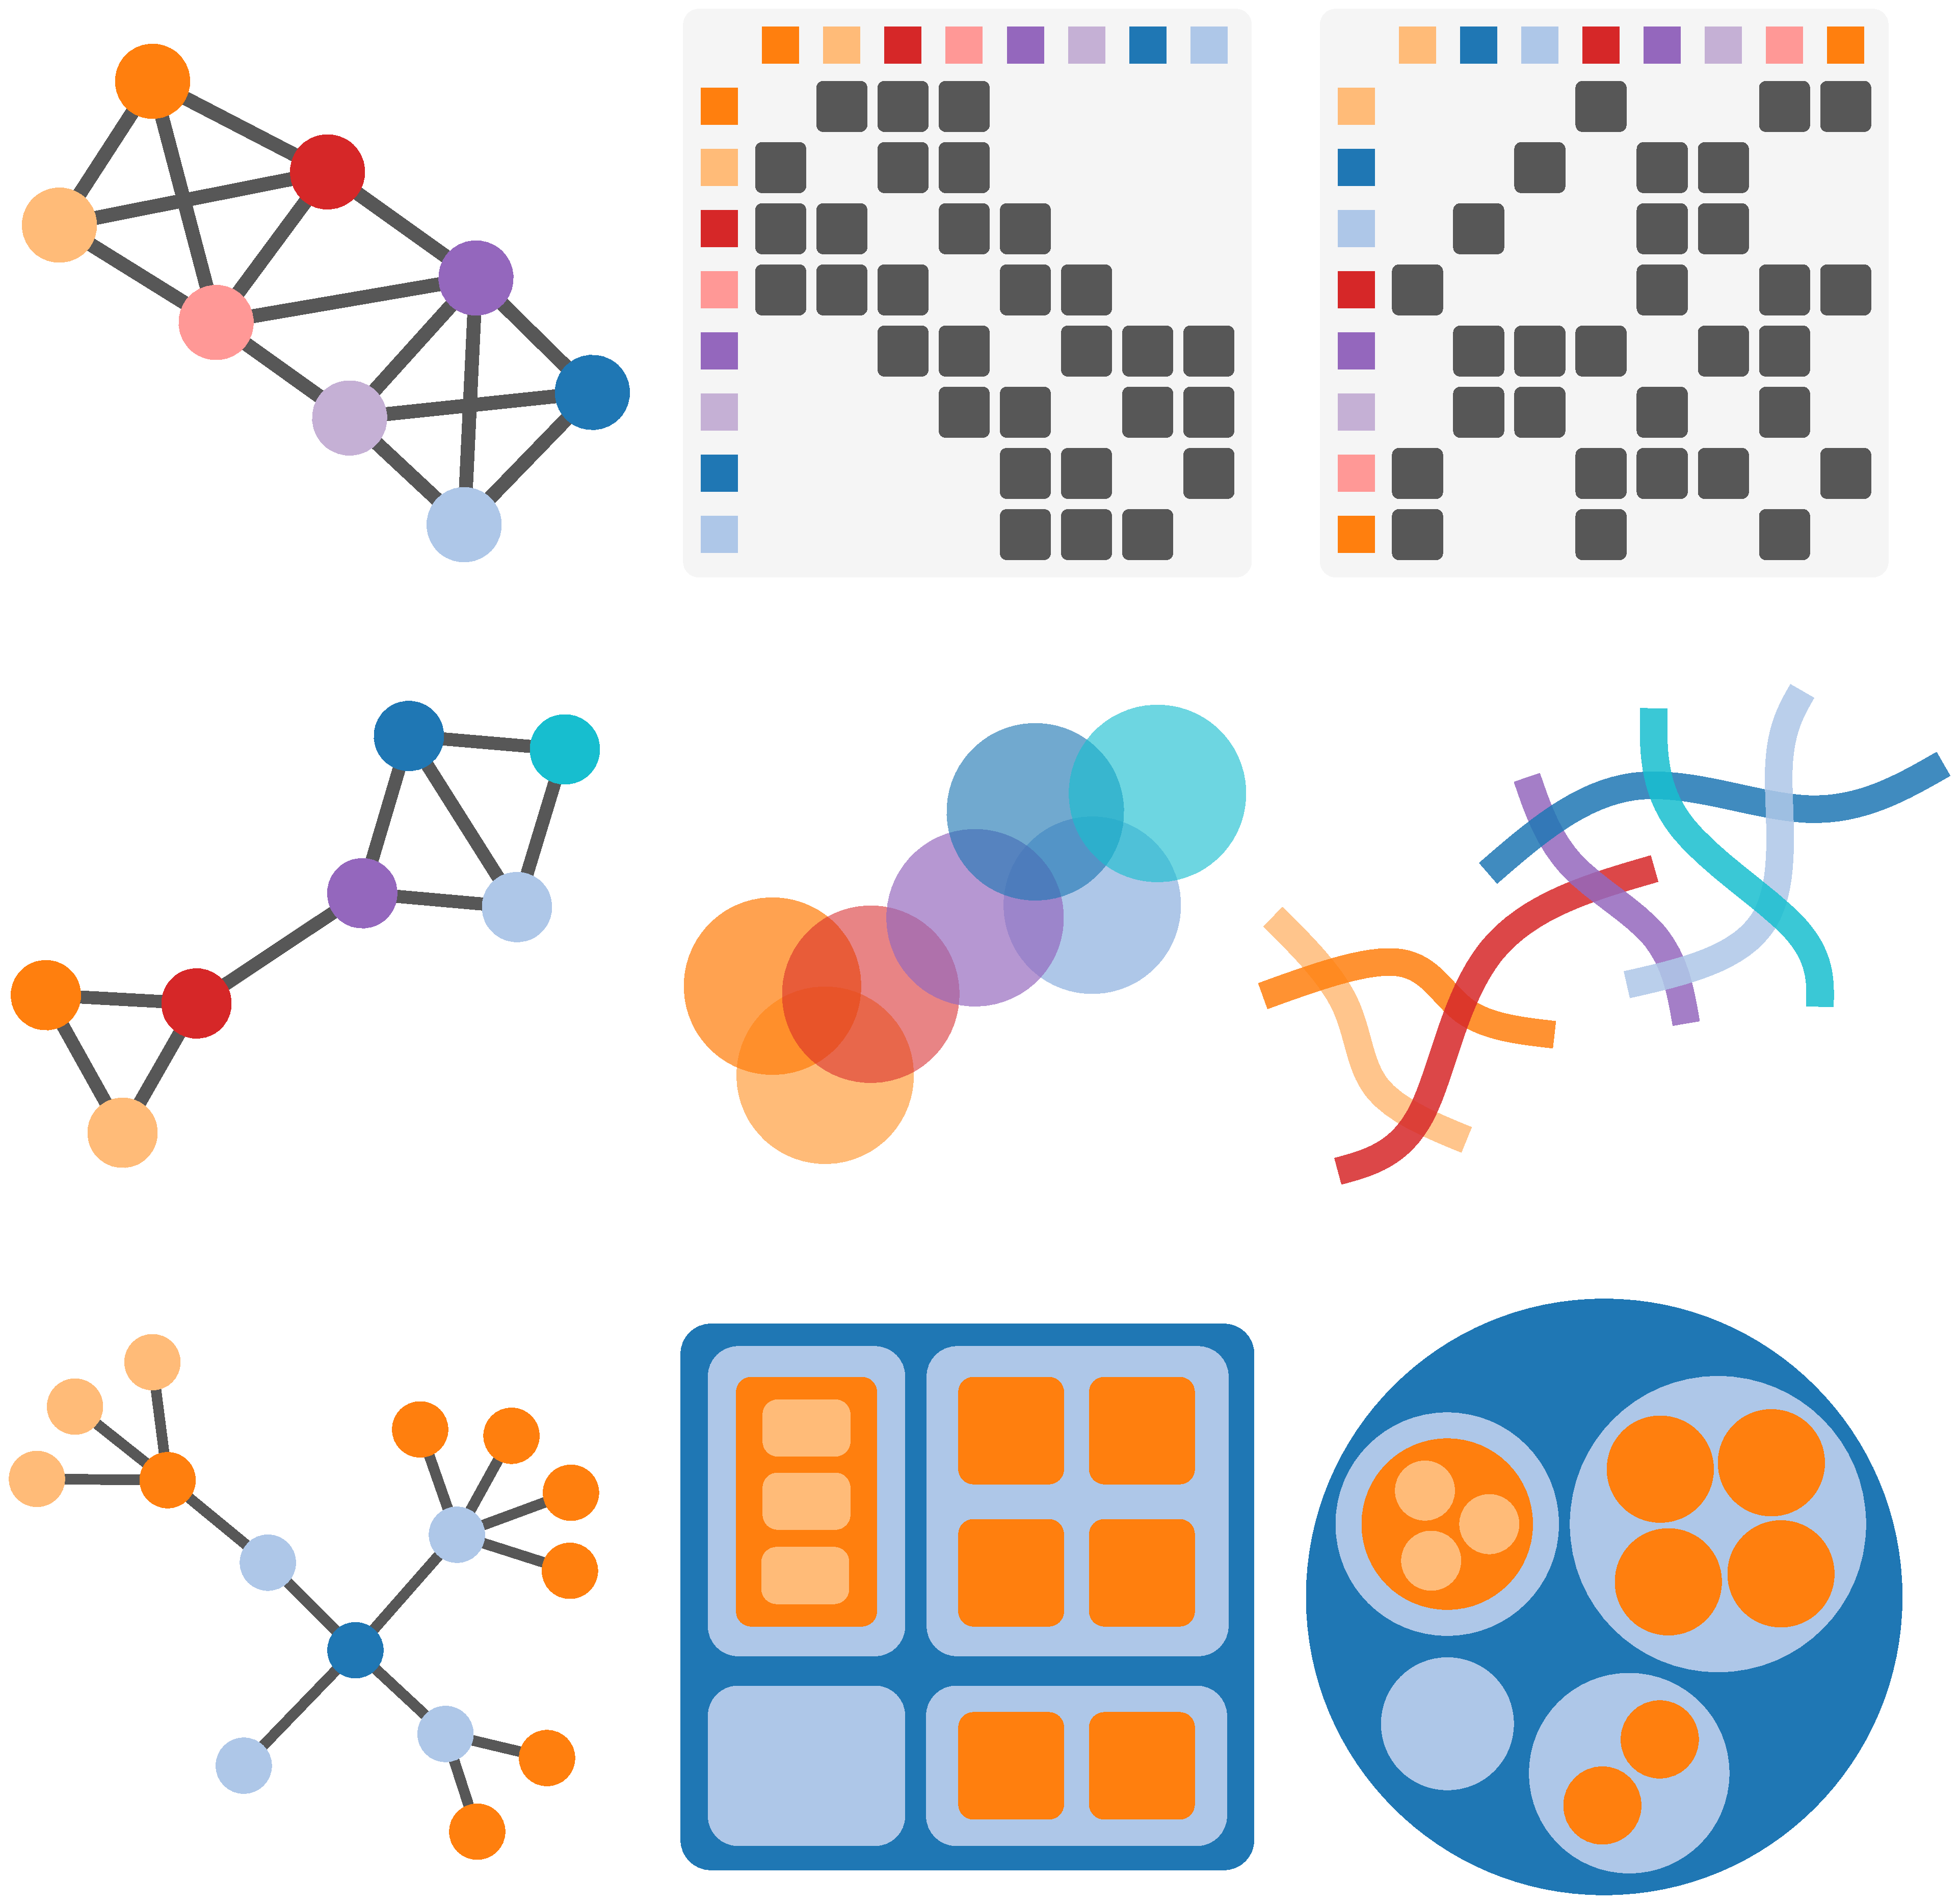
\includegraphics[width=\textwidth]{stress/representations.pdf}
  \caption[A gallery of graph representations]{A gallery of different graph representations, where left column contains node-link diagrams for three different graphs, and each row shows the same graph but in different representations. The top row shows matrix plots with rows ordered nicely and shuffled; the middle shows disc and string intersection graphs; the bottom shows rectangular and circle packed treemaps.
  }
  \label{fig:graph_representations}
\end{figure}

If one were to ask a random group of people to draw a network on a piece of paper, it is likely that most would draw dots to represent the nodes, and lines joining the dots to represent the edges. This is a representation so intuitive that it is often synonymous with the abstract concept of a network entirely.
This is the reason why this `join-the-dots' representation, known as the node-link diagram, is the most commonly studied and applied \citep{Ghoniem2004}, and is also why it has been chosen for the purposes of this thesis.

The contribution of this first chapter is entirely focused on algorithms for positioning the nodes in a node-link representation, specifically through the numerical optimisation of a popular objective function known as \emph{stress} \citep{Zheng2019Stochastic}.
However, it is useful to have an idea of the other possible graph representations in order to gain a broader view of what network visualisation can be. A classical example of this includes the \emph{matrix plot}, which is a grid where each vertex is represented by a row and a column, and each edge is a dot filled in at the intersection of a row and column \citep{Liiv2010}.
Specialised types of networks can also have similarly specialised representations. Trees, for example, can be depicted as packed rectangles \citep{Johnson1991} or circles \citep{Wang2006}, in what are known as \emph{treemaps}.
Graphs with low \emph{boxicity}, such as food webs \citep{Eklof2013}, can be drawn as \emph{intersection graphs} of overlapping lines or rectangles or cuboids.\footnote{Or hypercuboids, although the usefulness of that for visualisation is likely limited.}
A related and more common example is the \emph{disc graph}, where nodes are represented by circles and edges exist if the circles overlap. This sees widespread use as a Venn diagram, but usually without the connotation of network structure.
A more obscure example is \emph{string graphs}, where each vertex is represented by a (possibly curved) line, and edges exist between vertices whose lines intersect.

A gallery of such examples can be seen in Figure~\ref{fig:graph_representations}.
Each of these each of these representations has its unique benefits and downsides: matrix plots can show a very dense amount of data in a small space, but are very dependent on the ordering of rows and columns \citep{Liiv2010}, as it can be seen in Figure~\ref{fig:graph_representations} that shuffling the order of rows and column can completely hide the underlying structure. A survey of algorithms that can be used to find insightful orderings can be found in \citet{Bach2016}.
The intersection-style graphs are intuitive and do not require edges to be explicitly drawn, thus saving on visual clutter. However they cannot be drawn for all graphs for either the circle \citep{McDiarmid2014} or string \citep{Schaefer2003} representations.
Treemaps effectively convey the idea of a hierarchy, where the root node completely envelops each of its children in a recursive manner. On their own they can only visualise trees, but have been effectively used in conjuction with clustering algorithms to apply them to general graphs; examples of this include \emph{graph thumbnails} \citep{Yoghourdjian2018}, or \emph{power graph decomposition} \citep{Dwyer2014} which will be studied later in Chapter~\ref{chap:power}, Section~\ref{sec:power_graph}.
  
% Because of the difference between the abstract mathematical structure of a network and its representation within a visualisation, the abstract structure itself will henceforth be referred to a graph comprised of vertices and edges, and its representation a a network comprised of nodes and links.\footnote{This is in line with the terminology chosen by the \emph{International Symposium on Graph Drawing and Network Visualisation} to separate its theoretical and applied submission tracks, and so I will attempt to adopt it here. However the distinction between the two can sometimes become blurred depending on the context.}

Even within the subfield of node-link diagrams, there is a wide variety of options available.
Examples include \emph{arc} or \emph{chord diagrams}, where nodes are placed on a line or around a circle, respectively. Links are then added by drawing the eponymous arcs or chords between nodes.
A method that has recently gained popularity is the \emph{hive plot}, a simple but effective variant of parallel coordinate plots \citep{Krzywinski2012}, which places nodes on radial lines to draw curves between them, in a similar fashion to radar charts \citep{Porter2018}. An important subtlety is that each node may or may not be placed on more than one line, and the order in which the nodes are spread across the line is also a conscious choice. This customisability is where the power of such a method lies.

Hopefully the above examples give a taste of how varied the representation of a graph can be, even if the work in this thesis focuses its attention solely on the node-link diagram. The remainder of this chapter will specifically concern the \emph{layout} of nodes in such a visualisation.
And while there will be a focus on automatic node layout, it is worth noting that how humans tackle the problem has also been studied empirically \cite{Purchase2010, Purchase2014}.

\section{Background}
\label{sec:nodes_background}
The formal study of node-link diagrams dates back to least the 1920s. For example, F\'ary's theorem is a famous proof that any planar graph, defined as a graph that can be drawn without any intersecting links, can always be drawn in a planar way without needing links to be curved. This proof is attributed to \citet{Fary1948}, and was independently discovered by a host of other authors in the same era \citep{Steinitz1922, Wagner1936, Koebe1936, Stein1951}.
The ensuing development of actual \emph{algorithms} for network layout emerged around the 1960s, with its seminal work widely attributed to the barycentre algorithm of \citet{Tutte1963}.

Tutte's algorithm is very simple, and boils down to solving a system of linear equations, each of which strives to set a single node to the barycentre (i.e.\ mean position) of its neighbours. This is defined as 
\begin{equation}
  \mathbf{X}_i = \frac{1}{|N(i)|}\sum_{j\in N(i)}\mathbf{X}_j
\label{eq:tutte}
\end{equation}
where $\mathbf{X}_i$ is the $i^\text{th}$ row of the $|V|\times k$ matrix $\mathbf{X}$, with $V$ being the set of vertices in the graph and $k$ the dimensionality of the layout (usually two); $N(i)$ is the set of vertices neighbouring $i$.
Throughout this chapter, $\mathbf{X}$ will represent the coordinates of nodes in a layout.
Note that a necessary initial step is to fix the position of a selection of nodes around the boundary of the drawing, in order to avoid the trivial solution of placing all nodes in the same position.
The powerful insight that Tutte revealed with his algorithm was a remarkable mathematical theorem attached to it. He proved that this barycentre algorithm will always produce a planar drawing, in the specific case that the graph is planar and tri-connected (i.e.\ the graph cannot be disconnected by removing two vertices, no matter which two are removed).

This algorithm has served as the springboard for two main branches of network layout algorithms. Since planarity has been shown to be one of, if not the most important markers for readability in node-link diagrams \citep{Purchase1997}, the first branch is a line of planarity-based algorithms which can guarantee planar node layouts. Examples include the algorithm of \citet{Read1987} which recursively removes nodes and adds dummy edges to maintain a triangulated graph at each step.  A problem with this method and Tutte's is \emph{node resolution}, which means that nodes may be placed exponentially close to each other, rendering the graph impossible to read in certain areas.
A breakthrough for this problem came in 1990 by \citet{DeFraysseix1990} who described the first layout algorithm to achieve an asymptotically optimal node resolution of an $\mathcal{O}(|V|\times |V|)$ grid, and in linear time \citep{Chrobak1995}.
An example output of this algorithm can be seen in Figure~\ref{fig:dFPP}, which works by constructing a \emph{canonical ordering} of the graph \citep{Zhang2005} to order nodes on the x-axis, and from there y-axis positions can be chosen such to avoid crossings.

\begin{figure}
    \centering
    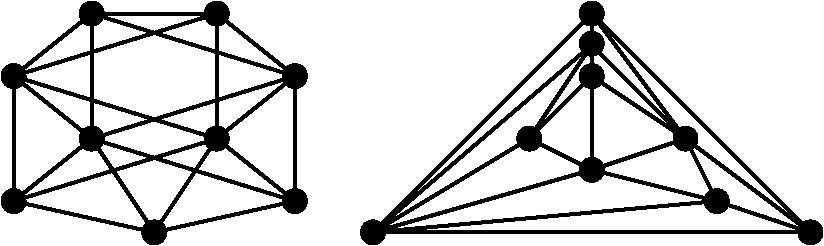
\includegraphics[width=\textwidth]{stress/dFPP.pdf}
    \caption[An example output of a planarity-based algorithm]{A graph with nodes positioned symmetrically (left) and without crossings (right) from using the algorithm of \citet{DeFraysseix1990}. Despite the planarity of the output, the poor angular resolution makes the drawing more difficult to read.}
    \label{fig:dFPP}
\end{figure}

Improvements and refinements have been made with this algorithm in mind \citep{Zhang2005}, but such methods suffer from poor \emph{angular resolution}, which means that adjacent edges form small angles between each other, another property that has been shown to negatively impact the readability of layouts \citep{Purchase1997}.
Such an example of poor angular resolution is illustrated in Figure~\ref{fig:dFPP}.
This issue exists until this day \citep{Eades2012}, and is a primary reason why most network visualisation software uses algorithms based on a second, less mathematically rigorous branch of algorithms also inspired by Tutte.

This second branch comes from an intuitive interpretation of Tutte's algorithm: that each edge is analogous to a spring of zero natural length, where the solution to Tutte's system of linear equations can be seen as the point at which the elastic energy of these springs, according to Hooke's law \citep{Hooke1678}, is minimised. This energy is defined as
\begin{equation}
  \mathrm{energy}(\mathbf{X}) = \sum_{\{i,j\}\in E}||\mathbf{X}_j-\mathbf{X}_i||^2
\label{eq:tutte_energy}
\end{equation}
where $E$ is the set of all edges. Differentiating with respect to the position of a single node $\mathbf{X}_i$ results in
\begin{equation}
  \frac{d}{d\mathbf{X}_i}\mathrm{energy}(\mathbf{X}) = \sum_{j\in N(i)}-2(\mathbf{X}_j-\mathbf{X}_i)
\label{eq:tutte_force}
\end{equation}
where it can be seen that setting the left-hand side to zero results in Equation~\eqref{eq:tutte}, corresponding to an embedding of minimum global energy in the system.

This interpretation has been taken and advanced to alleviate the resolution problem present in planarity based methods, by introducing the trade-off of foregoing mathematical rigour. 
This is done by using human intuition to formulate variations on Equation~\eqref{eq:tutte_energy}, in what are known as \emph{force-directed} algorithms.

\subsection{\texorpdfstring{\st{Force-directed}{ Optimisation algorithms}}{}}
\label{sec:force_background}
This section will present an overview of the various methods that have sprouted from this second branch of algorithms, around which the work in this chapter is based. All such algorithms will also be framed within the wider context of \emph{optimisation}, a framework which will tie together otherwise loosely-connected threads in a logical taxonomy.\footnote{This interpretation of framing the layout problem as optimisation is far from new, for example a technique known as simulated annealing has been applied to graph drawing since the 90s \citep{Davidson1996} which is strongly rooted within the field of optimisation. However it is important to acknowledge the word `force' as a slight misnomer, as physical simulations are not used in their implementation, a fact also emphasised by \citet{Fruchterman1991} in their description of their popular layout method. `Force-inspired' may have made for better terminology.}
It will also lead more cogently into the novel contributions described in Section~\ref{sec:sgd}.
A gallery of the algorithms to be described here is presented in Figure~\ref{fig:misc_force_layouts}.

\begin{figure}
  \centering
%   \makebox[\textwidth][c]{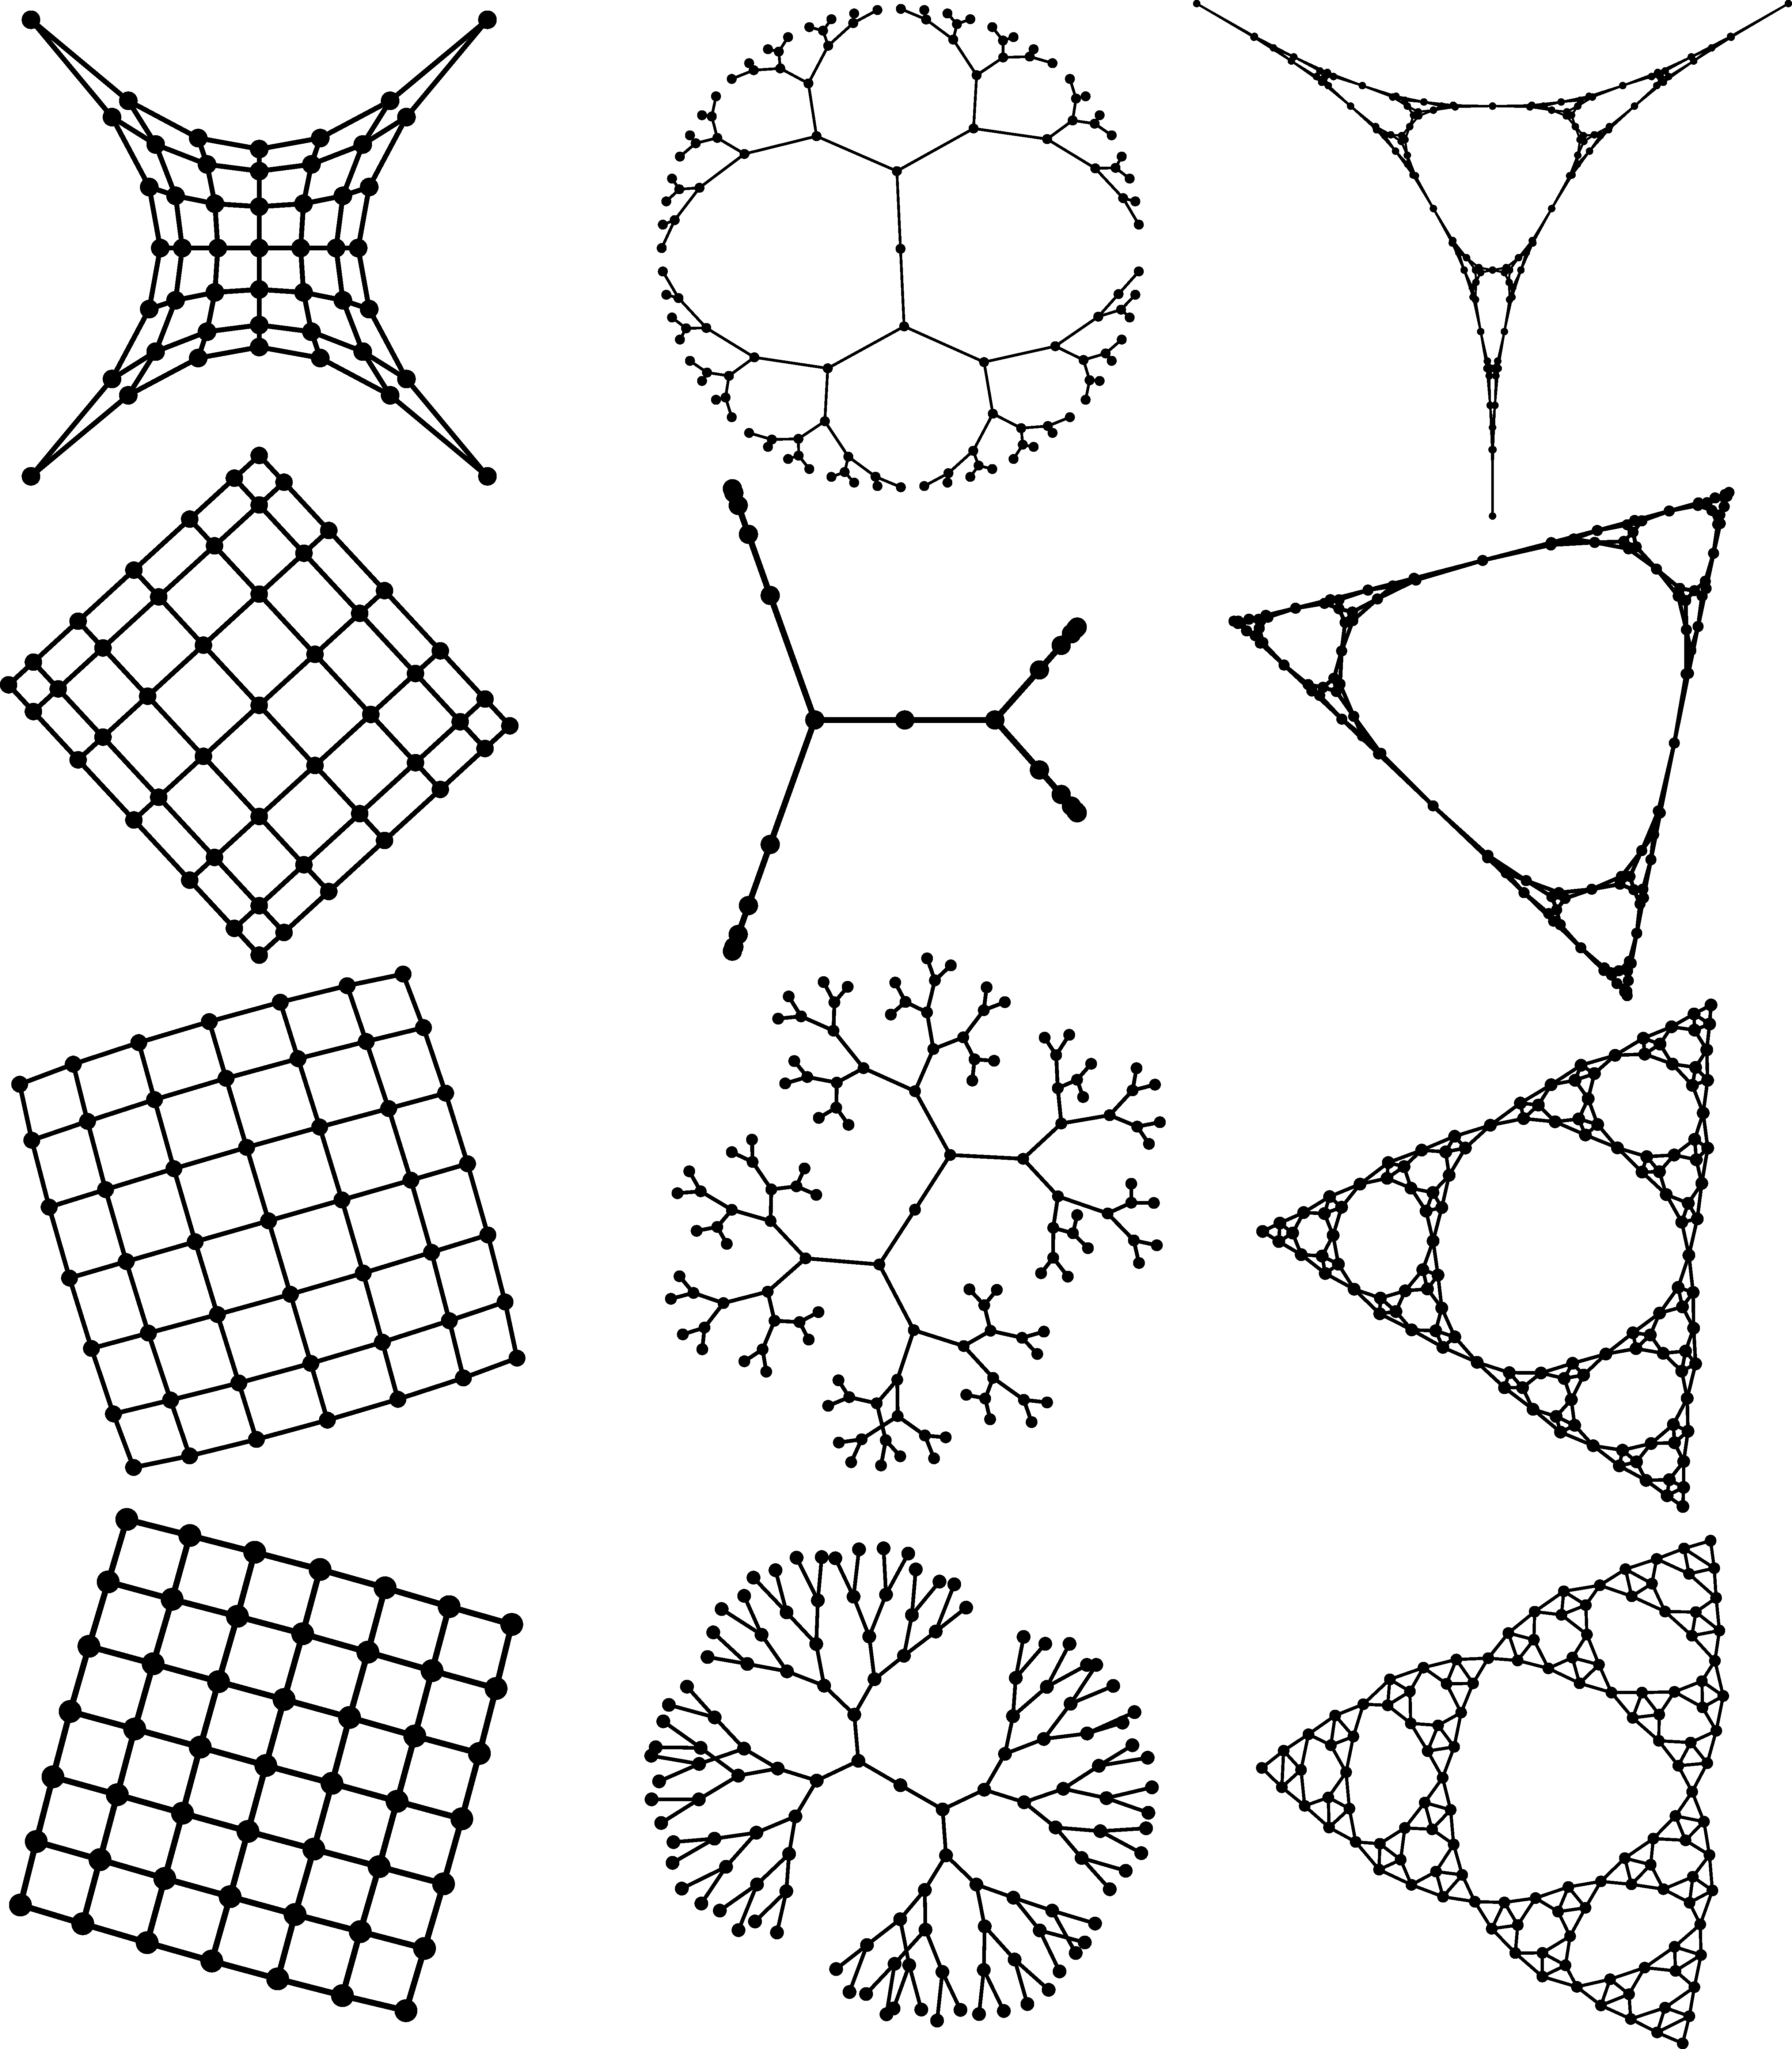
\includegraphics[width=1.1\textwidth]{stress/force.pdf}}
  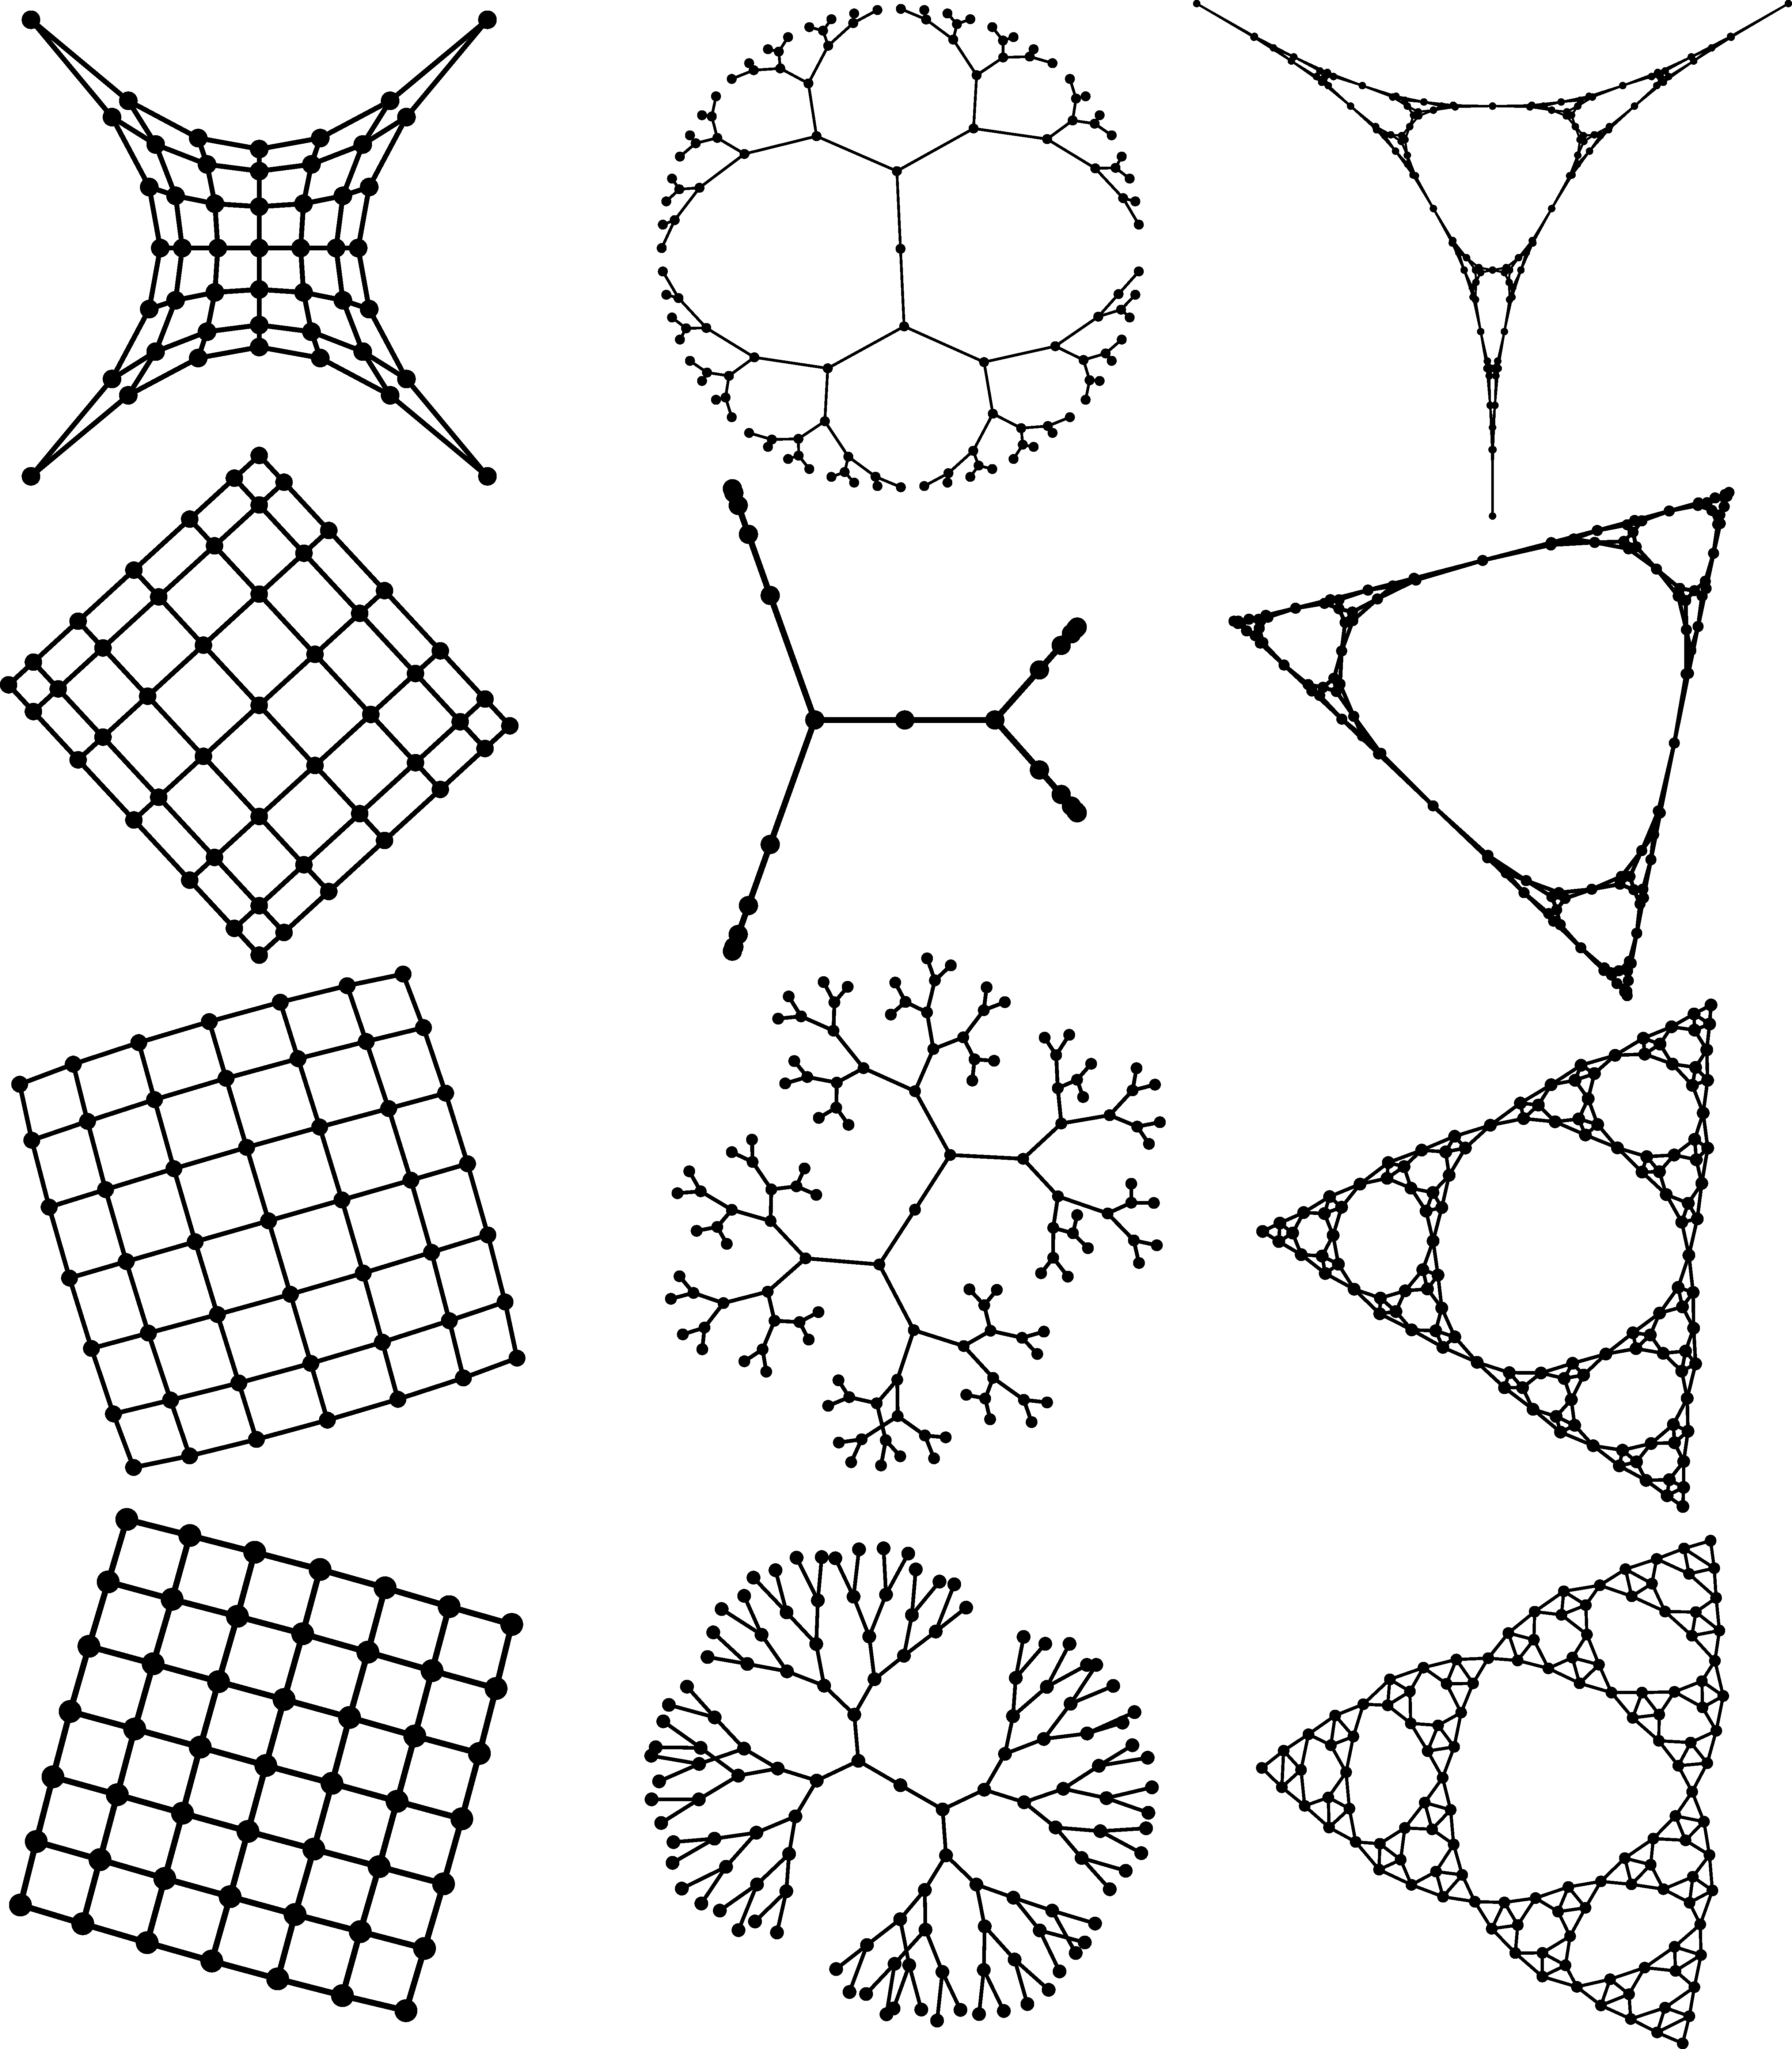
\includegraphics[width=1.03\textwidth]{stress/force.pdf}
  \caption[A gallery of node layout methods]{
  Three graphs visualised with four different force-directed algorithms from Section~\ref{sec:force_background}. Graphs are, from left to right, a grid of width seven, a binary tree of depth seven, and a Sierpi\'nski triangle \citep{Sierpinski1915} with five sub-triangle recursions.
  The algorithms used are, from top to bottom, Tutte~\eqref{eq:tutte}, spectral~\eqref{eq:spectral}, Eades~\eqref{eq:eades}, and stress~\eqref{eq:stress}.
  The nodes pinned to the edge of the layout for Tutte are the four corners of the grid, all leaf nodes in the binary tree, and the three corners of the biggest Sierpi\'nski triangle.}
  \label{fig:misc_force_layouts}
\end{figure}

The earliest of these algorithms was developed by \citet{Eades1984} who, inspired by techniques for positioning transistors on integrated circuits \citep{Quinn1979}, made two modifications. The first was to alter the edge springs in order to give them a non-zero natural length, avoiding having to fix an often arbitrary selection of nodes around the boundary. The second was to introduce a repulsive force between pairs of non-adjacent vertices to spread nodes evenly around the drawing.
The combination of these forces on a single node $i$ is defined as
\begin{equation}
  \frac{d}{d\mathbf{X}_i}\mathrm{energy}(\mathbf{X}) = -\sum_{j\in N(i)}c_1\log(||\mathbf{X}_j-\mathbf{X}_i||)\overrightarrow{\mathbf{X}_{ij}}
  + \sum_{j\notin N(i)}\frac{c_2}{||\mathbf{X}_j-\mathbf{X}_i||^2}\overrightarrow{\mathbf{X}_{ij}}
  \label{eq:eades}
\end{equation}
where $\overrightarrow{\mathbf{X}_{ij}} = \frac{\mathbf{X}_j-\mathbf{X}_i}{||\mathbf{X}_j-\mathbf{X}_i||}$, i.e.\ the normalised vector pointing from $i$ to $j$, and $c_1$ and $c_2$ are constant parameters determining the relative strengths of the forces. The first summation defines the `springs', where the logarithm attempts to maintain the spring at unit length by flipping to negative if the node pair gets too close together.\footnote{Hooke's law was abandoned by Eades because ``\emph{Experience shows that Hookes Law (linear) springs are too strong when the vertices are far apart; the logarithmic force solves this problem}" \citep{Eades1984}.}
The second summation is the repulsive force, which always pushes $i$ away from $j$ if there does not exist an edge between them, and decays according to an inverse square function analogous to charged electrons obeying Coulomb's law \citep{Coulomb1785}.

There are two important aspects to notice here. The first is that the left-hand side is not the energy itself, but its derivative. The second is that this derivative can no longer be straightforwardly solved as in Equation~\eqref{eq:tutte} because it has become \emph{non-linear}. How then is energy minimised? Through a method known as \emph{gradient descent}, which is as simple as iteratively moving nodes in the direction opposite to the derivative in Equation~\eqref{eq:eades} according to
\begin{equation}
  \mathbf{X}_i \leftarrow -\eta\, \frac{d}{d\mathbf{X}_i}\mathrm{energy}(\mathbf{X})
\label{eq:gradient_descent}
\end{equation}
where $\eta$ is a constant parameter.
This operation, despite its simplicity, is theoretically proven to find a minimal energy embedding \citep{Cauchy1847}, although it is important to note that this embedding may not be globally optimal because the energy function defined by~\eqref{eq:eades} is \emph{non-convex} and therefore may contain many \emph{local minima}. Many of the concepts introduced in this paragraph will be elaborated upon in Section~\ref{sec:stress_background}.

This optimisation through gradient descent interpretation is not how this type of algorithm is commonly presented, as  force-directed algorithms are often categorised into two families: force-balancing and energy-minimising models \citep{Ortmann2017, Brandes2001Physical}.
Eades' model fits into the former, while others fit into the latter by directly defining an energy function such as in~\eqref{eq:tutte_energy}.
Energy is then minimised by gradient descent as in Equation~\eqref{eq:gradient_descent} or by another optimisation technique, as will be further elaborated upon in Section~\ref{sec:stress_background}.
With the view that the action of `force-balancing' is equivalent to gradient descent on another energy function, however, it is made clear that the two families are equivalent in the sense that both strive for the same goal: minimising energy.

This optimisation-centric viewpoint also allows a variety of linear algebra-based methods to be grouped into the same taxonomy.
The algorithm of \citet{Harel2004} first embeds a graph in a high-dimensional space, determined by a covariance matrix of graph-theoretic or shortest-path distances, and then finds an optimal projection down to two dimensions by finding the eigenvectors of this this matrix. This is commonly known as principal components analysis (PCA) \citep{Pearson1901}.
The \emph{classical scaling} approach of \citet{Brandes2007Eigensolver} is based on constructing the high-dimensional embedding from a double centered \emph{distance matrix} between high-dimensional points and then performing PCA. The intuition behind this method is that it optimises the inner product between low- and high-dimensional distances.
The \emph{spectral} approach, originally developed by \citet{Hall1970} and largely ignored by the field until \citet{Koren2003}, uses a graph Laplacian as the high-dimensional matrix instead of shortest-paths, upon which PCA is again applied. This approach is particularly closely related to Tutte's algorithm, which in fact utilises the same graph Laplacian when solving for Equation~\eqref{eq:tutte}.
The eigenvalue approach even optimises the same energy function, but requires the variance of the embedding to be non-zero, thereby avoiding the need to fix certain nodes around the boundary \citep{Koren2003}.
In mathematical terms, its energy upon a single dimension of the layout in the column vector $\mathbf{x}$ can be derived as
\begin{align}
\begin{split}
  \mathrm{energy}(\mathbf{x}) &= \sum_{\{i,j\}\in E}w_{ij}(\mathbf{x}_j-\mathbf{x}_i)^2\\
  \mathrm{var}(\mathbf{x}) &= \frac{1}{n}\sum_i(\mathbf{x}_i-\overline{\mathbf{x}})^2 = 1
\end{split}
\label{eq:spectral}
\end{align}
where $w_{ij}$ is an optional weight given to each edge (previously all set to 1 in~\eqref{eq:tutte}) and $\overline{\mathbf{x}}$ is the mean of $\mathbf{x}$. The one-dimensional layout that minimises energy is equal to the second smallest eigenvector of the Laplacian matrix $\mathbf{L}$, defined such that
\begin{equation}
  \mathbf{x}^T\mathbf{Lx} = \mathrm{energy}(\mathbf{x})
  \label{eq:spectral_laplacian}
\end{equation}
where $\mathbf{x}^T$ denotes the transpose of $\mathbf{x}$. Subsequent dimensions are found by calculating subsequent eigenvectors of $\mathbf{L}$, often through power iteration \citep{Koren2003}.
All of these methods boil down to finding the eigendecomposition of a certain matrix which describes the graph in a different way, and each set of eigenvectors describes an \emph{optimal projection} into a lower dimension.

The linear nature of such methods is a double-edged sword, as it allows them to be calculated and/or approximated quickly and precisely, but they all suffer from the same issue that resulting layouts under-represent local detail \citep{Brandes2008}, especially in examples such as the binary tree in Figure~\ref{fig:misc_force_layouts}, second row. However their effectiveness at capturing global structure consistently has led to them being commonly used as an initialisation step \citep{Brandes2008, Dwyer2009}.

Circling back to non-linear methods, there have been many attempts at improving Eades' original formulation. A widely-used alternative, developed in 1991, is the method of \citet{Fruchterman1991} who revert springs back to having a natural length of zero, but balance this out by applying the repulsive force between all pairs of vertices. Counter-intuitively, increasing the number of repulsive terms also makes the summation more efficient to calculate, by taking inspiration from techniques used in physical simulations \citep{Hachul2004, Hu2005}. More detail on scaling layout algorithms to large graphs can be found in Section~\ref{sec:large_graphs}.
Another notable attempt came from \citet{Frick1995}, who altered the calculations to never require a square root operation, and introduced a number of extra heuristics to speed up the convergence of the optimisation procedure in Equation~\eqref{eq:gradient_descent}. These heuristics were introduced on an intuitive and ad hoc basis, but have been shown to greatly speed up convergence in practice \citep{Brandes2001Physical}.
% \begin{equation}
%   \frac{d}{d\mathbf{X}_i}\mathrm{energy}(\mathbf{X}) = -\sum_{j\in N(i)}\frac{c^2}{||\mathbf{X}_j-\mathbf{X}_i||}\overrightarrow{\mathbf{X}_{ij}}
%   + \sum_{j:j\neq i}\frac{||\mathbf{X}_j-\mathbf{X}_i||^2}{c}\overrightarrow{\mathbf{X}_{ij}}
% \end{equation}

The energy function that will become the focus for the rest of this chapter is known as \emph{stress}, and was popularised within the context of graph layout in by \citet{Kamada1989}. Its energy is defined as
\begin{equation}
  \mathrm{stress}(\mathbf{X}) = \sum_{\{i,j\}:i<j}w_{ij}(||\mathbf{X}_j-\mathbf{X}_i||-d_{ij})^2
\label{eq:stress}
\end{equation}
where $w_{ij}$ and $d_{ij}$ are constants specific to each term in the summation. The intuition behind this formulation is that there are Hooke's law springs attached between all pairs of vertices, not just those connected by edges. Each of these springs is of natural length $d_{ij}$ and of stiffness $w_{ij}$. In practice, $d_{ij}$ is usually set to the shortest-path distance between vertices, and $w_{ij}$ is almost always set to $d_{ij}^{\text{--}2}$ in order to suppress the contribution from long-range springs that would otherwise obfuscate local detail \citep{Brandes2008}.

The derivative of this equation is non-linear, like in Equation~\eqref{eq:eades} or in \citet{Fruchterman1991, Frick1995}, and so cannot be solved exactly using linear solvers like for Equations~\eqref{eq:tutte_energy} or~\eqref{eq:spectral}.
% However an immediate benefit to this formulation is that there are no extra input parameters for the user to decide, since $w_{ij}$ and $d_{ij}$ are both dependent on the structure of the graph itself.
However, stress as an energy function is known to produce high-quality layouts \citep{Brandes2008}. This is partly because it manages to avoid the \emph{peripheral effect} \citep{Hu2005}, a common visual artifact of many force-directed methods where repulsive forces tend to push nodes towards the boundary of the layout.
This can be seen in Figure~\ref{fig:misc_force_layouts} for Eades' method; the grid on the left bulges slightly, while the binary tree and Sierpi\'nski triangle underrepresent local detail.
Stress avoids this by forgoing repulsive forces entirely in Equation~\eqref{eq:stress}, as can also be seen in the bottom row in Figure~\ref{fig:misc_force_layouts}.

Stress also does not require extra input parameters such as those in Equation~\eqref{eq:eades} because $d_{ij}$ and $w_{ij}$ are both derived from the structure of the graph itself.
However, it is known to be difficult to optimise due to an abundance of local minima \citep{DeLeeuw1988, Gansner2004}, and also does not scale well to larger graphs due to the quadratic number of terms in the summation \citep{Brandes2008, Hu2005}.

The subsequent content of this chapter will aim at addressing these issues through the application of an algorithm known as \emph{stochastic gradient descent} (SGD) to minimise Equation~\eqref{eq:stress}. Before describing the algorithm itself however, a history of other methods used to minimise stress will first be outlined.

\subsection{Multidimensional scaling}
\label{sec:stress_background}
Equation~\eqref{eq:stress} was first utilised in a domain unrelated to graphs, but still for the purpose of visualisation, known as \emph{multidimensional scaling} (MDS). As the name implies, this involves taking high-dimensional data and scaling it down to fewer dimensions, usually to two or three.

The difficulty in this task can be illustrated through a simple example: the humble tetrahedron. The task at hand is to find an `ideal' drawing of the tetrahedron, where `ideal' is defined as having each of its edges drawn with equal length. When one tries to draw such a configuration on a piece of (two-dimensional) paper, it quickly becomes clear that it is not possible.
Even for such a small graph with only four vertices, there are too few dimensions available to provide sufficient degrees of freedom.
%\footnote{The rate at which such a problem can get out of hand is known as the \emph{curse of dimensionality} \citep{Friedman2001Local}, which is range of phenomena caused by the exponential growth of a given problem space relative to each additional input dimension}
The next logical question is: what layout gets as close as possible to this ideal?

Multidimensional scaling (MDS) is a technique to solve exactly this type of problem, that attempts to minimize the disparity between ideal and low-dimensional distances.
% but generalized to any number of input or output dimensions.
This is done by defining an equation to \emph{quantify} the error in a layout, and then minimizing it in a similar fashion to the algorithms above in Section~\ref{sec:force_background}. While this equation can come in many forms \citep{Cox2000}, stress as in Equation~\eqref{eq:stress} is the most commonly used for graph layout \citep{Brandes2008}, for the reasons described at the end of the previous section.

The use of Equation~\eqref{eq:stress} was popularized for graph layout by \citet{Kamada1989} who minimized the function using a localized 2D Newton-Raphson method, while within the MDS community \citet{Kruskal1964Optimizing} originally used gradient descent \citep{Kruskal1964Numerical}. This was later improved upon by \citet{DeLeeuw1988} with a method known as \emph{majorization},
which minimizes a complicated function by iteratively finding the 
true minima of a series of simpler functions, each of which touches the 
original function and is an upper bound for it \citep{Cox2000}.
This was applied to graph layout by \citet{Gansner2004} and has been the state-of-the-art for the past decade.

\subsection{Majorization}
\label{sec:majorization}
Majorization is the algorithm that will be used throughout this chapter as the benchmark against which the performance of SGD will be assessed.
It works by first finding a Laplacian matrix $\mathbf{L}^w$, defined as
\begin{equation}
  \mathbf{L}_{ij}^w =
  \begin{cases}
    \;-w_{ij} & \text{if }\;i\neq j\\
    \;-\sum_{k\neq i}\mathbf{L}_{ik}^w & \text{if }\;i=j
  \end{cases}
  \label{eq:major_Lw}
\end{equation}
and then another Laplacian matrix $\mathbf{L^X}$, defined as
\begin{equation}
  \mathbf{L}_{ij}^\mathbf{X} =
  \begin{cases}
    \;-w_{ij}d_{ij}||\mathbf{X}_i-\mathbf{X}_j||^{-1} & \text{if }\;i\neq j\\
    \;-\sum_{k\neq i}\mathbf{L}_{ik}^\mathbf{X} & \text{if }\;i=j.
  \end{cases}
  \label{eq:major_LX}
\end{equation}
It can be shown that the equation
\begin{equation}
  \mathbf{L}^w\mathbf{x}^\prime = \mathbf{L^Xx}
  \label{eq:major_linear}
\end{equation}
where $\mathbf{x}$ and $\mathbf{x}^\prime$ are column vectors that represent single dimensions of the full layouts $\mathbf{X}$ and $\mathbf{X}^\prime$ respectively, guarantees that $\text{stress}(\mathbf{X}^\prime) \leq \text{stress}(\mathbf{X})$ \citep{Gansner2004}.
The optimisation process is then performed simply by solving Equation~\eqref{eq:major_linear} as a system of linear equations, with $\mathbf{x}^\prime$ as the column of unknowns being solved for. This is repeated in an iterative manner, where $\mathbf{x}^\prime$ is computed in one iteration and then used as $\mathbf{x}$ in the next, until the algorithm can no longer improve the value of stress by more than a certain threshold. Note that $\mathbf{L}^w$ only needs to be computed once, but $\mathbf{L}^\mathbf{X}$ must be recalculated on every iteration.

Additionally in practice, the position of the first vertex is fixed to the origin, and the first row and column of $\mathbf{L}^w$ are removed, as well as the first row of the vector $\mathbf{L^Xx}$. This is in order to remove translational invariance from the solution, which allows for fast linear equation solving methods to be applied to solve Equation~\ref{eq:major_linear}.
In particular, \citet{Gansner2004} recommend \emph{Cholesky factorization} \citep{Press2007Cholesky} or the \emph{conjugate gradient} method \citep{Press2007Conjugate}, both of which will be tested later in Section~\ref{sec:sgd_experiment}. 

\citet{Gansner2004} also described another \emph{local} method for solving Equation~\ref{eq:major_linear}, where the system of equations is solved for just one vertex at a time. This is done by setting the position of vertex $i$ to
\begin{equation}
  \mathbf{x}_i^\prime = \frac{\sum_{j\neq i}w_{ij}(\mathbf{x}_j + d_{ij}(\mathbf{x}_i - \mathbf{x}_j)||\mathbf{X}_i - \mathbf{X}_j||^{-1})}{\sum_{j\neq i}w_{ij}}
  \label{eq:major_local}
\end{equation}
and is also guaranteed to monotonically decrease stress \citep{Gansner2004}. This local method will also be tested later in Section~\ref{sec:sgd_experiment}, and will furthermore be important when considering large graphs in Section~\ref{sec:large_graphs}.

\subsection{Constraint relaxation}
\label{sec:wcr_story}
The origin of the novel contributions in this chapter is rooted in constrained graph layout, where a relaxation algorithm, here referred to as \emph{constraint relaxation}, has gained popularity due to its simplicity and versatility \citep{Dwyer2009,Bostock2011}. This algorithm will provide the context to the geometric interpretation of SGD that will be leveraged to make the modifications in Section~\ref{sec:sgd}.

Constraint relaxation was first introduced in video game engines as a technique to quickly approximate the behavior of cloth, which is modeled as a planar mesh of vertices that maintains its edges at a fixed length.
A full physics simulation would represent each edge as a stiff spring, summing up and integrating over the resulting forces, but a realistic piece of cloth contains too many edges for this to be feasible.

To avoid this bottleneck, \citet{Jakobsen2001} introduced the idea of considering each edge independently, moving a single pair of vertices at a time.
While this is a rather simple and perhaps naive idea, in practice the solution converges in very few iterations.

This was utilized by \citet{Dwyer2009}, who used the method in conjunction with any standard force-directed layout to achieve effects such as making edges point downwards, or fixing cycles around the edge of a wheel. To define it properly in the case of maintaining a distance $d_{ij}$ between the coordinates of two nodes $\mathbf{X}_i$ and $\mathbf{X}_j$, this \emph{constraint} can be written as
\begin{equation}
  ||\mathbf{X}_i - \mathbf{X}_j|| \leftarrow d_{ij}
  \label{eq:constraint}
\end{equation}
and is \emph{satisfied} by moving $\mathbf{X}_i$ and $\mathbf{X}_j$ in opposite directions by a vector
\begin{equation}
  \mathbf{r} = \frac{||\mathbf{X}_i - \mathbf{X}_j||-d_{ij}}{2}\frac{\mathbf{X}_i - \mathbf{X}_j}{||\mathbf{X}_i - \mathbf{X}_j||}.
  \label{eq:satisfaction}
\end{equation}
This can be seen as a diagram in Figure~\ref{fig:satisfaction}, and is analogous to decompressing an infinitely stiff spring of length $d_{ij}$.

\begin{figure}
  \centering
  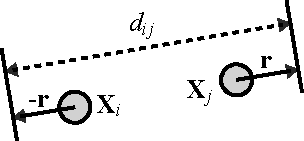
\includegraphics[width=.5\textwidth]{stress/satisfaction.pdf}
  \caption[Illustration of the distance constraint in Equation~\ref{eq:constraint}]{Satisfaction of the distance constraint described by Equation~\eqref{eq:constraint}.}
  \label{fig:satisfaction}
\end{figure}

Rewriting Equation~\eqref{eq:stress} as
\begin{gather}
\label{stress-terms}
\mathrm{stress}(\mathbf{X}) = \sum_{i<j} Q_{ij}(\mathbf{X}),\\
\label{qij}
Q_{ij}(\mathbf{X}) = w_{ij}(||\mathbf{X}_i - \mathbf{X}_j|| - d_{ij})^2,
\end{gather}
it can be seen that if every term $Q_{ij}$ in the summation is satisfied as a constraint~\eqref{eq:constraint}, then the total stress is zero, corresponding to an ideal layout. 
This is exactly the idea behind the method that will be studied here --- a constraint is placed on every possible pair of vertices, and then satisfied one by one as above.

However zero stress is almost always impossible, for the same reasons that the aforementioned tetrahedron cannot be embedded in 2D. In such situations, simply satisfying constraints does not lead to convergence, but the rest of this chapter will be dedicated to describing a simple extension that not only converges but, remarkably, also minimises stress.

\newpage
\section{Stochastic gradient descent}
\label{sec:sgd}
The remaining content of this chapter will describe the novel application of stochastic gradient descent (SGD) to minimise stress. SGD is a method widely used in other fields, most notably in machine learning \citep{Bottou2012}, but not previously applied to minimise Equation~\ref{eq:stress}. 
SGD approximates the gradient of a sum of functions using the gradient of its individual terms. For stress in particular, this has an intuitive geometric interpretation of moving a single pair of vertices at a time; this interpretation allows for a simple modification to the optimisation step which help to avoid local minima and speed up convergence. The benefits of SGD over majorization will be shown through experiment.

The modifications required to the constraint relaxation described above can be understood by first noticing that satisfying a constraint is equivalent to moving both vertices in the direction of the gradient of a stress term $Q_{ij}$
\begin{equation}
  \label{gradient}
  \frac{\partial Q_{ij}}{\partial\mathbf{X}_i}=\frac{\partial}{\partial\mathbf{X}_i}w_{ij}(||\mathbf{X}_i - \mathbf{X}_j|| - d_{ij})^2 = 4w_{ij}\mathbf{r}.
\end{equation}
The full gradient $\partial Q_{ij}/\partial\mathbf{X}$ can be written as
\begin{equation}
  \frac{\partial Q_{ij}}{\partial\mathbf{X}_k}=
  \begin{cases}
    \;4w_{ij}\mathbf{r} & \mbox{if $k=i$} \\
    \;-4w_{ij}\mathbf{r} & \mbox{if $k=j$} \\
    \;0 & \mbox{otherwise.} \\
  \end{cases}
\end{equation}
Recall that standard force-directed methods use (non-stochastic) gradient descent, following Equation~\eqref{eq:gradient_descent}, and that this involves taking a step in the opposite direction to the derivative of the entire summation at once.
The change required for stochastic gradient descent is as simple as doing the same thing, but to a single term at a time.

Specifically, this involves repeatedly selecting a single term $Q_{ij}$ and applying the iterative formula $\mathbf{X}\leftarrow \mathbf{X}-\eta\nabla Q_{ij}(\mathbf{X})$.
Note that since this gradient is zero with respect to all $\mathbf{X}_k$ other than $\mathbf{X}_i$ and $\mathbf{X}_j$, it suffices to update the positions of $\mathbf{X}_i$ and $\mathbf{X}_j$ by
\begin{equation}
  \begin{bmatrix}\mathbf{X}_i\\\mathbf{X}_j\end{bmatrix}
  \leftarrow
  \begin{bmatrix}\mathbf{X}_i\\\mathbf{X}_j\end{bmatrix}+
  \begin{bmatrix}\Delta \mathbf{X}_i\\\Delta \mathbf{X}_j\end{bmatrix}
  =
  \begin{bmatrix}\mathbf{X}_i\\\mathbf{X}_j\end{bmatrix}-
  4w_{ij}\eta
  \begin{bmatrix}\mathbf{r}\\-\mathbf{r}\end{bmatrix}.
  \label{eq:SGD_step}
\end{equation}

The constraint relaxation of the previous section is therefore equivalent to a special case of SGD where $w_{ij}=1$ and $\eta=1/4$.\footnote{This equivalence to stochastic gradient descent was not known for a long time, as neither \citet{Jakobsen2001} nor \citet{Dwyer2009} classified the algorithm correctly. In fact, not even my supervisors and I knew that this was SGD in the first version of this paper we submitted to a journal, where we chose the name \emph{weighted constraint relaxation}.}
Additionally in this case, a gradual reduction in the step size $\eta$ is necessary to make the process converge, since not all terms can be simultaneously minimised. This will be further elaborated in Section~\ref{sec:annealing}, and the problem can be interpreted in the context of stress as each edge of the aforementioned tetrahedron satisfying its constraint one by one as in Figure~\ref{fig:satisfaction}, but never finding a configuration where all are satisfied at the same time.

Writing $\mu=4w_{ij}\eta$ as the coefficient of $\mathbf{r}$, it can be seen that $Q_{ij}\leftarrow 0$ when $\mu=1$ and decreases monotonically from $\mu=0$ to $\mu=1$.
In other words, the exact step size required to optimally minimise each term $Q_{ij}$ can always be instantly known. This is the geometric interpretation that allows for a modification to SGD, specific to the context of stress. It involves setting a hard upper limit of $\mu\leq 1$:
\begin{equation}
  \begin{aligned}
    \Delta\mathbf{X}_i &= -\Delta\mathbf{X}_j = -\mu\, \mathbf{r},\\
    \mu&=\min\{\,w_{ij}\eta, \, 1\,\}
  \end{aligned}
  \label{eq:mu}
\end{equation}
where the constant factor of $4$ has been absorbed into $\eta$ for brevity.
This modified algorithm makes updates that are identical to standard SGD when $\eta$ is sufficiently small, at
\begin{equation}
  % \eta<1/\max_{ij} w_{ij}.
  \eta<\frac{1}{w_{\max}}.
  \label{eq:eta-sufficiently-small}
\end{equation}
Since this will always eventually be the case because $\eta$ tends to zero, it has the same asymptotic convergence properties as standard SGD, which will be discussed in Section~\ref{sec:annealing}.

\begin{figure}
  \centering
  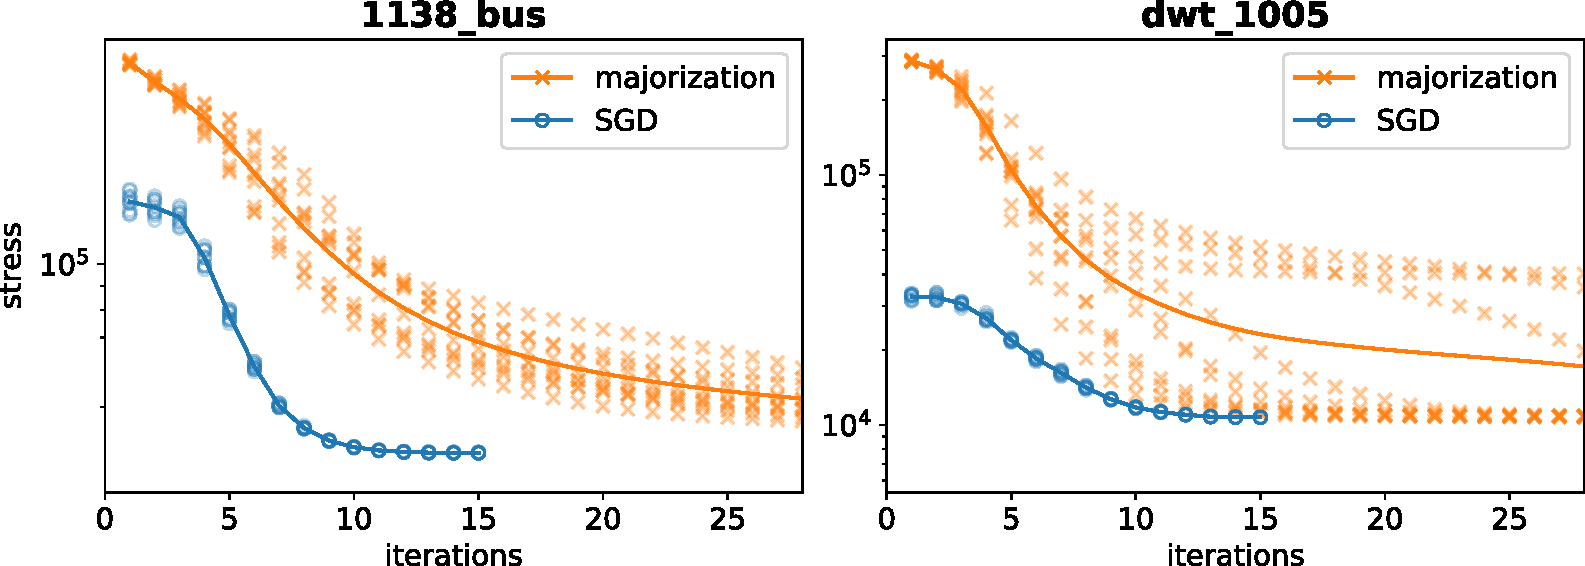
\includegraphics[width=.9\textwidth]{stress/iterations.pdf}
  \caption[Results against majorization for \texttt{1138\_bus} and \texttt{dwt\_1005}]{Plots of stress for SGD and majorization on the graphs \texttt{1138\_bus} and \texttt{dwt\_1005}, each initialized randomly within a 1$\times$1 square.
  The circles and crosses show stress on each iteration over 10 runs, with the line running through the mean.
  Initial stress values are omitted.
  SGD is clearly more consistent, always reaching lower stress levels than majorization ever manages in hundreds of iterations on \texttt{1138\_bus}.
  They both reach the same overall minimum on the more mesh-like \texttt{dwt\_1005}, but majorization often gets stuck on a particularly dangerous local minimum, shown by its diverging paths.
  A more detailed timing analysis on a wide variety of other examples can be seen in Section~\ref{sec:sgd_experiment}.
  }
  \label{fig:stress_plots}
% \end{figure}
  \vspace*{\floatsep}
  \vspace*{\floatsep}
% \begin{figure}
  \removeAlgorithmFigureError
  \begin{algorithm}[H]
    \SetKwProg{SGD}{SGD}{}{}
    \SetKwInOut{Input}{inputs}
    \SetKwInOut{Output}{output}
    \SetKwFor{ForEach}{foreach}{:}{}
    \SetKwFor{For}{for}{:}{}
    \SetKwIF{If}{ElseIf}{Else}{if}{:}{elif}{else}{}
    
    \SGD{\emph{\textbf{(}}$G$\emph{\textbf{):}}}{
      \Input{graph $G=(V,E)$}
      \Output{$k$-dimensional layout $\mathbf{X}$}
      
      $d_{ij} \leftarrow \textsc{ShortestPaths}(G)$
      \label{code:sgd:bacon}
      
      $\mathbf{X} \leftarrow \textsc{Rand}(|V|,k)$
      \label{code:sgd:init}
      
      \For{$\eta$ \emph{in \textsc{AnnealingSchedule}()}}{
      \label{code:sgd:annealing}
      
        \ForEach{$\{i,j\}:i<j$ \emph{in random order}}{
        
          $\mu \leftarrow w_{ij} \eta$
          
          \If{$\mu > 1$}{ \label{code:sgd:if1}
              $\mu \leftarrow 1$ \label{code:sgd:if2}
          }
          
          $\mathbf{r} \leftarrow \frac{||\mathbf{X}_i - \mathbf{X}_j||-d_{ij}}{2}\frac{\mathbf{X}_i - \mathbf{X}_j}{||\mathbf{X}_i - \mathbf{X}_j||}$
          
          $\mathbf{X}_i \leftarrow \mathbf{X}_i - \mu\,\mathbf{r}$
          \label{code:sgd:satisfaction1}
          
          $\mathbf{X}_j \leftarrow \mathbf{X}_j + \mu\,\mathbf{r}$
          \label{code:sgd:satisfaction2}
        }
      }
    }
    \caption{Stochastic Gradient Descent}
    \label{alg:sgd}
  \end{algorithm}

  \caption[Pseudocode for stochastic gradient descent]{
  Pseudocode for the algorithm described in Section~\ref{sec:sgd}.
  The results in this paper initialize positions randomly within a 1$\times$1 square on line~\ref{code:sgd:init}.
  The annealing schedule on line~\ref{code:sgd:annealing} is explained in Section~\ref{sec:annealing}.
  }
  \label{fig:pseudo_sgd}
\end{figure}

Introducing this upper limit on $\mu$ allows for much larger initial step sizes than standard SGD, yielding much faster convergence without needing to worry about divergence due to \emph{exploding gradients} \citep{Goodfellow2016}. It will be shown     by experiment that this results in state-of-the-art performance for a wide range of graphs (except for a single specific case, see Section~\ref{sec:sgd_experiment}).
In addition, \emph{random reshuffling} of terms is used unless otherwise stated; see Section~\ref{sec:randomisation} for further elaboration. A full pass through all the terms $Q_{ij}$ will be referred to as an \emph{iteration}, while a single application of Equation~\eqref{eq:SGD_step} will be referred to as a \emph{step}.
From now on, the modified SGD algorithm simply as SGD.

Plots of stress achieved using SGD compared to majorization are presented briefly in Figure~\ref{fig:stress_plots}, and in more detail in Section~\ref{sec:sgd_experiment}. Pseudocode is shown in Algorithm~\ref{alg:sgd}, Figure~\ref{fig:pseudo_sgd}.
All results have vertex positions initialized uniformly randomly within a 1$\times$1 square, with optimisation performed using C\# running in Visual Studio, on an Intel Core i7-4790 CPU with 16GB of RAM.
Unless stated otherwise, graph data is from the SuiteSparse Matrix Collection \citep{Davis2011}.

\subsection{Step size annealing}
\label{sec:annealing}
The process of gradually reducing the step size over the course of the optimisation, so that the process can converge, will be referred to as an \emph{annealing schedule}.
Choosing a good annealing schedule $\eta$ is crucial to the performance of SGD in all contexts \citep{Darken1992}, and a typical implementation can involve complex algorithms for tuning the step size to the problem at hand \citep{Ruder2016}.
Most of these methods do not apply here for two reasons. First, due to the limit on the step size in Equation~\eqref{eq:mu}, much larger step sizes than standard SGD would allow can and will be used. Second, many of these methods use previous gradients to inform the step size; only positions of the two vertices directly involved are updated, so storing and applying previous gradients is inefficient to the point of increasing the asymptotic complexity of the algorithm.

Even ignoring such adaptive methods, the full (infinite) space of possible annealing schedules is too large to investigate in its entirety, and results can even differ depending on the input graph. A limited subset of possible schedules will therefore be tested, taking the mean final stress across a wide range of graphs as the performance criterion
(the full set of graphs considered in Section~\ref{sec:sgd_experiment}).
Two use cases will be considered: one where time is a limiting factor and so the number of iterations is fixed, and another where the algorithm may continue until the layout has converged to within a desired accuracy.

\subsubsection{Fixed number of iterations}
The schedules to be studied here will consider step size that starts at a maximum value $\eta=\eta_\mathrm{max}$ at the first iteration $t=0$, and decreases monotonically to $\eta=\eta_\mathrm{min}$ at the final iteration $t=t_\mathrm{max}-1$.
Large values of $\eta$ result in all $\mu$ capped at 1, and very small values will result in little to no movement of vertices. Because the useful range exists only in between these extremes, $\eta$ is set to
\begin{equation}
  \eta_{\max} = \frac{1}{w_{\min}} \,,\;\; \eta_{\min} = \frac{\varepsilon}{w_{\max}}.
  \label{eq:etamaxmin}
\end{equation}
In this case $w_{ij} = d_{ij}^{-2}$ so $w_{\min}$ is inversely proportional to the diameter of the graph $d_{\max}$, and $w_{\max}$ to the smallest edge length $d_{\min}$.
This choice of $\eta_{\max}$ ensures that all $\mu = 1$ for the first iteration, resulting in the constraint relaxation described in Section~\ref{sec:wcr_story} applied to all pairs of vertices. The choice of $\eta_{\min}$ ensures that even the strongest constraints reach a small value of $\mu = \varepsilon$ for the final iteration.

\begin{figure}
  \centering
  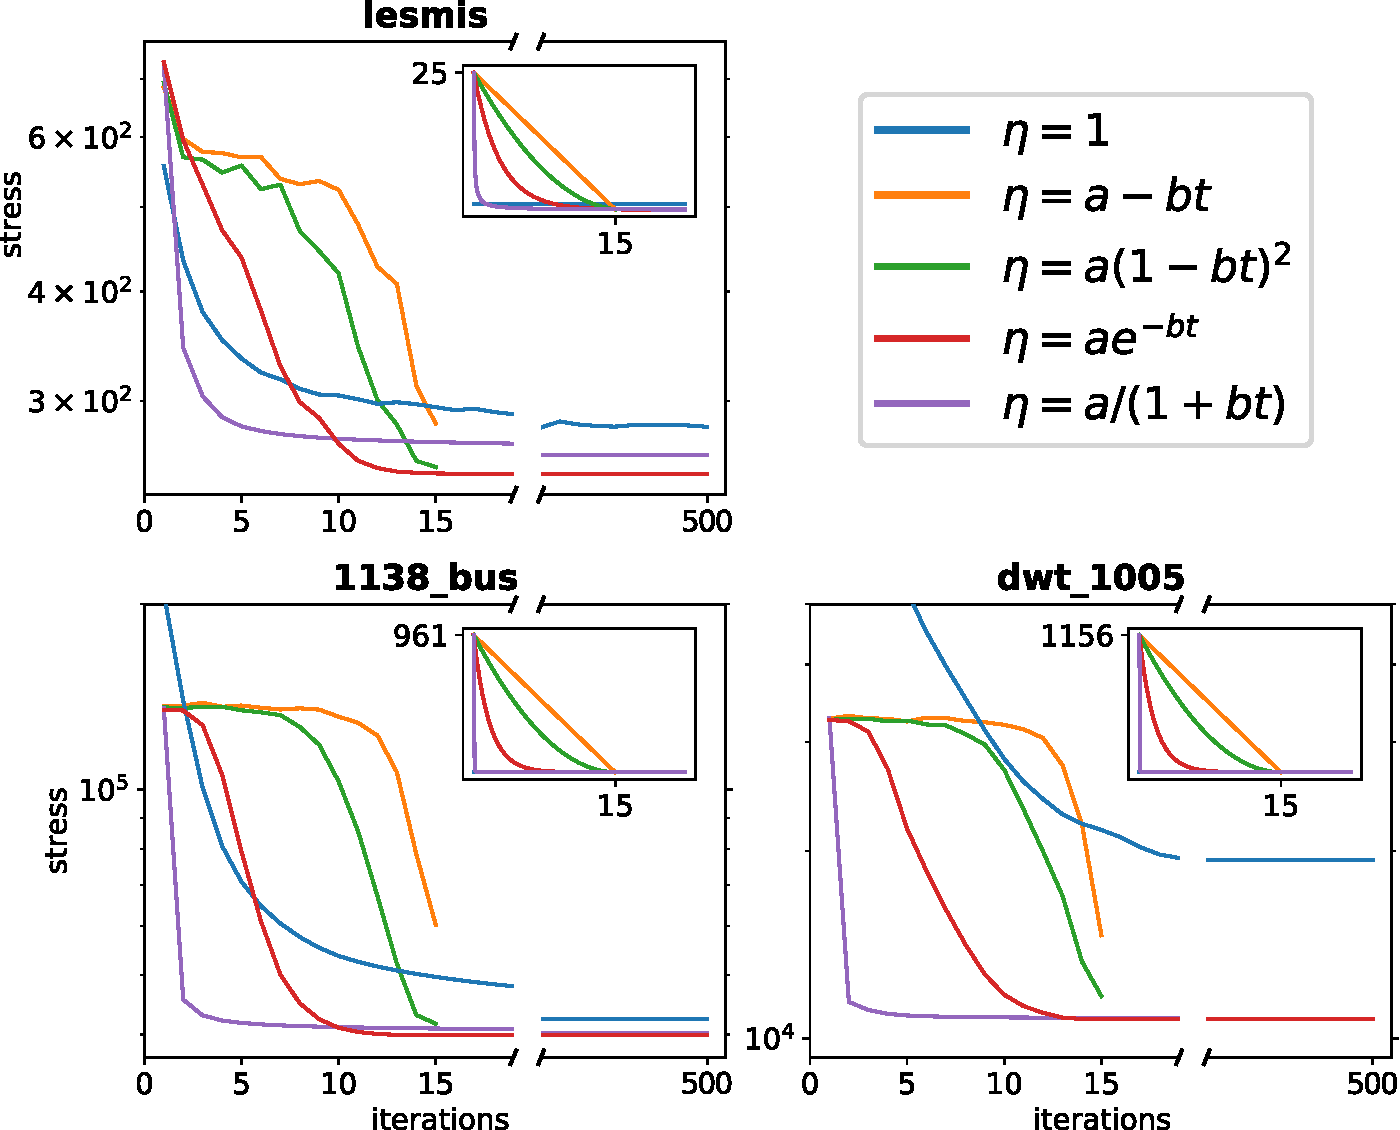
\includegraphics[width=.85\textwidth]{stress/cooling.pdf}
  \caption[A comparison of different annealing schedules]{Plots of mean stress against iterations over 25 runs for the annealing schedules discussed in Section~\ref{sec:annealing}, with $t_{\max}=15$ and $\varepsilon=0.1$ in all cases. The exact schedules used are shown inset in the top right of every plot.
  To approximate behavior given unlimited time, schedules were run for 500 iterations.
  }
  \label{fig:annealing}
% \end{figure}
  \vspace*{\floatsep}
  \vspace*{\floatsep}
% \begin{figure}
  \centering
  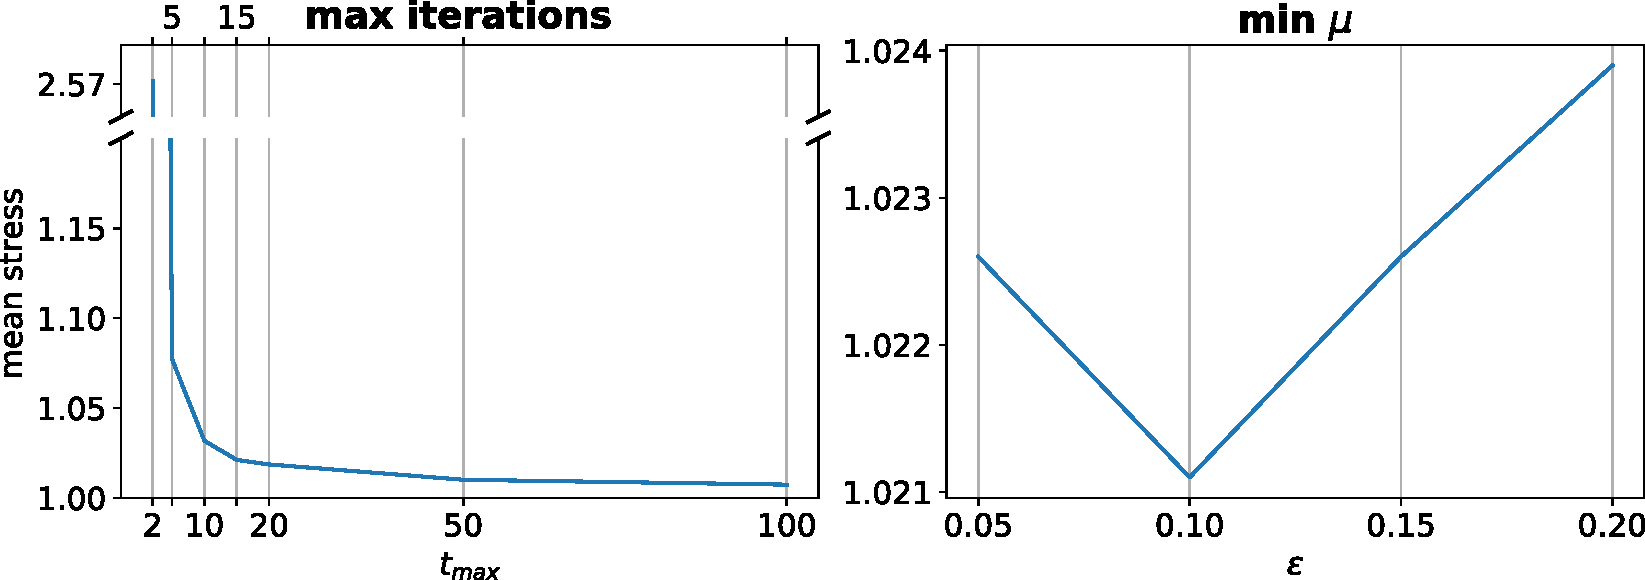
\includegraphics[width=.95\textwidth]{stress/parameters.pdf}
  \caption[A comparison of annealing schedule parameterisations]{Plots of mean stress over 25 runs on all graphs in Section~\ref{sec:sgd_experiment} when varying the parameters $t_{\max}$ or $\varepsilon$ on Equation~\eqref{eq:expodecay}, normalized to the best values over all runs from Figure~\ref{fig:systematic}.
  There are clear diminishing returns when increasing $t_{\max}$, so $t_{\max}=15$ was chosen as a trade-off between speed and quality.
  $\varepsilon=0.1$ is close to optimum for this value.
  }
  \label{fig:parameters}
\end{figure}

The performance was computed for various schedules $\eta(t)$ where $t$ is the iteration number, constrained to $\eta(0)=\eta_{\max}$ and $\eta(t_\mathrm{max}-1)=\eta_{\min}$ (except for the special case $\eta(t)=1$).
In each panel of Figure~\ref{fig:annealing} the form of the function $\eta(t)$ is varied for a fixed choice of $t_\mathrm{max}$ and $\varepsilon$, on various input graphs.
\texttt{1138\_bus} shows the typical behavior of $\eta= ae^{-bt}$ reaching lower stress and $\eta= a/(1+bt)$ never quite catching up; \texttt{lesmis} shows that this applies to smaller graphs as well; \texttt{dwt\_1005} emphasizes the importance of larger step sizes, as the constant $\eta=1$ struggles to ever jump over large local minima. Note that on this easier graph $\eta=a/(1+bt)$ is enough to reach good minima in very few iterations.

The best form of $\eta(t)$ appears to be the exponential decay given by the equation
\begin{equation}
  \eta_1(t) = \eta_{\max} e^{-\lambda t}.
  \label{eq:expodecay}
\end{equation}
In addition, the parameters $t_\mathrm{max}$ and $\varepsilon$ where varied for this form of $\eta(t)$ (see Figure~\ref{fig:parameters}).
Increasing $t_\mathrm{max}$ always improves the quality but also increases computation time, so $t_\mathrm{max}=15$ was chosen as a reasonable compromise between speed and quality.
With this number of iterations most of the gains had already been made and further ones gave diminishing returns, although for particular applications another choice may be more appropriate.
The right-hand side of Figure~\ref{fig:parameters} shows that the choice $\varepsilon=0.1$ appears to be close to optimal for this $t_{\max}$.

It is common in SGD to use a schedule
$\eta = \Theta(1/t)$ \citep{Darken1992},
however for the small number of iterations considered here, the large initial step sizes cause $\eta$ to decay too quickly in the beginning, leading to worse local minima. 
Exponential decay drops faster than $1/t$ as $t\rightarrow\infty$, but $1/t$ drops faster in early iterations given fixed values at $\eta(0)$ and $\eta(t_{\max}-1)$, as shown by the inset panels in Figure~\ref{fig:annealing}.

\subsubsection{Unlimited iterations}
The schedule described above works well in practice for a fixed number of iterations, but given more time it can be desirable to let the algorithm run for longer to produce an optimal layout.
Here a schedule will be described that is guaranteed to converge, with a stopping criterion to prevent the algorithm from wasting iterations on negligible movements.

A proof of convergence for SGD is well known in the machine learning literature \citep{Bottou2012}, and requires an annealing schedule that satisfies
\begin{equation}
  \sum_{t=0}^{\infty}\eta(t) = \infty
  \quad \text{and} \quad
  \sum_{t=0}^{\infty}\eta(t)^2 < \infty.
  \label{eq:convergence}
\end{equation}
This is guaranteed to reach global minima under conditions slightly weaker than convexity \citep{Bottou1998}.
Intuitively, the first summation ensures the decay is slow enough to reach the minimum no matter how far away it is initialized, and the second ensures fast enough decay to converge to, rather than bounce around the minimum \citep{Welling2011}.
In the context of non-convex functions, like the stress equation considered in this paper, such a proof only holds for convergence to a stationary point that may be a saddle \citep{Bottou1998}.
There is also recent work proving convergence to local minima in specific classes of non-convex functions \citep{Ge2015}.

Since a global minimum cannot be guaranteed with any choice of schedule, the best that can be done is to choose a schedule that will converge to a stationary point. A commonly used schedule that guarantees this is $\eta=\Theta(1/t)$, as this satisfies Equation~\eqref{eq:convergence}. However, in the previous section it was noted that this schedule gets stuck in poor local minima. A mixed schedule can therefore be used: when $t$ is small, $\eta(t)=\eta_1(t)$ follows the exponential schedule of the previous section, because in practice this avoids poor local minima; when $t$ is large this is switched to a $1/t$ schedule to guarantee convergence to a stationary point, following
\begin{equation}
  \eta_{2}(t + \tau) =
  \frac{w_{\max}^{-1}}{1+\lambda t}
  \quad \text{when}
  \quad t>\tau\: :\:
  \eta_{1}(\tau) = w_{\max}^{-1}.
\end{equation}
The cross-over value $\tau$ is the iteration at which the limit in Equation~\eqref{eq:mu} stops capping $\mu$ and the algorithm becomes standard SGD.
Since there are now more iterations to work with, $t_{\max}=30$ is chosen in order to further improve avoidance of local minima. This choice is sufficient to give even or better mean performance than majorization after convergence across every graph tested except for one (see Section~\ref{sec:sgd_experiment}), but again depending on the application another choice may be more suitable.

Finally, a suitable stopping criterion is needed to avoid the algorithm from never stopping, although in practice a hard upper limit for $t$ is also included. Since SGD does not guarantee the monotonic decrease of stress \citep{Darken1992}, the majorization heuristic adopted by \citet{Gansner2004} cannot be used, which stops when the relative change in stress drops below a certain threshold.
However it is guaranteed that each time a constraint is satisfied, its corresponding term within the summation does decrease.
How close the algorithm is to convergence is therefore estimated by tracking the maximum distance any vertex is moved by a single step over the previous iteration. The optimisation is stopped when this crosses a threshold
\begin{equation}
  \max||\Delta\mathbf{X}|| < \delta.
\end{equation}
A value of $\delta=0.03$ works well in practice, and is used for the results in Section~\ref{sec:sgd_experiment}.

Thus two schedules have been designed: one for a fixed number of iterations, and one that continues until convergence.
Results using both of these are presented in Section~\ref{sec:sgd_experiment}.
It is important to note that these schedules use simple heuristics, and the exact nature of the data will affect the results.
However they are robust across a wide variety of graphs, as all the results shown in this paper use these two schedules.

\subsection{Randomisation}
\label{sec:randomisation}
An important consideration is the order in which constraints are satisfied, as naive iteration can introduce biases that cause the algorithm to get caught in local minima.
The original method behind SGD, proposed by \citet{Robbins1951}, randomizes with replacement, meaning that a random term is picked every time with no guarantee as to how often a term will be picked. Some variants perform random reshuffling (RR) which guarantees that every term is processed once on each iteration. Under certain conditions it can be proven analytically that RR converges faster \citep{Gurbuzbalaban2019}, and the results here support this.

\begin{figure}
  \centering
  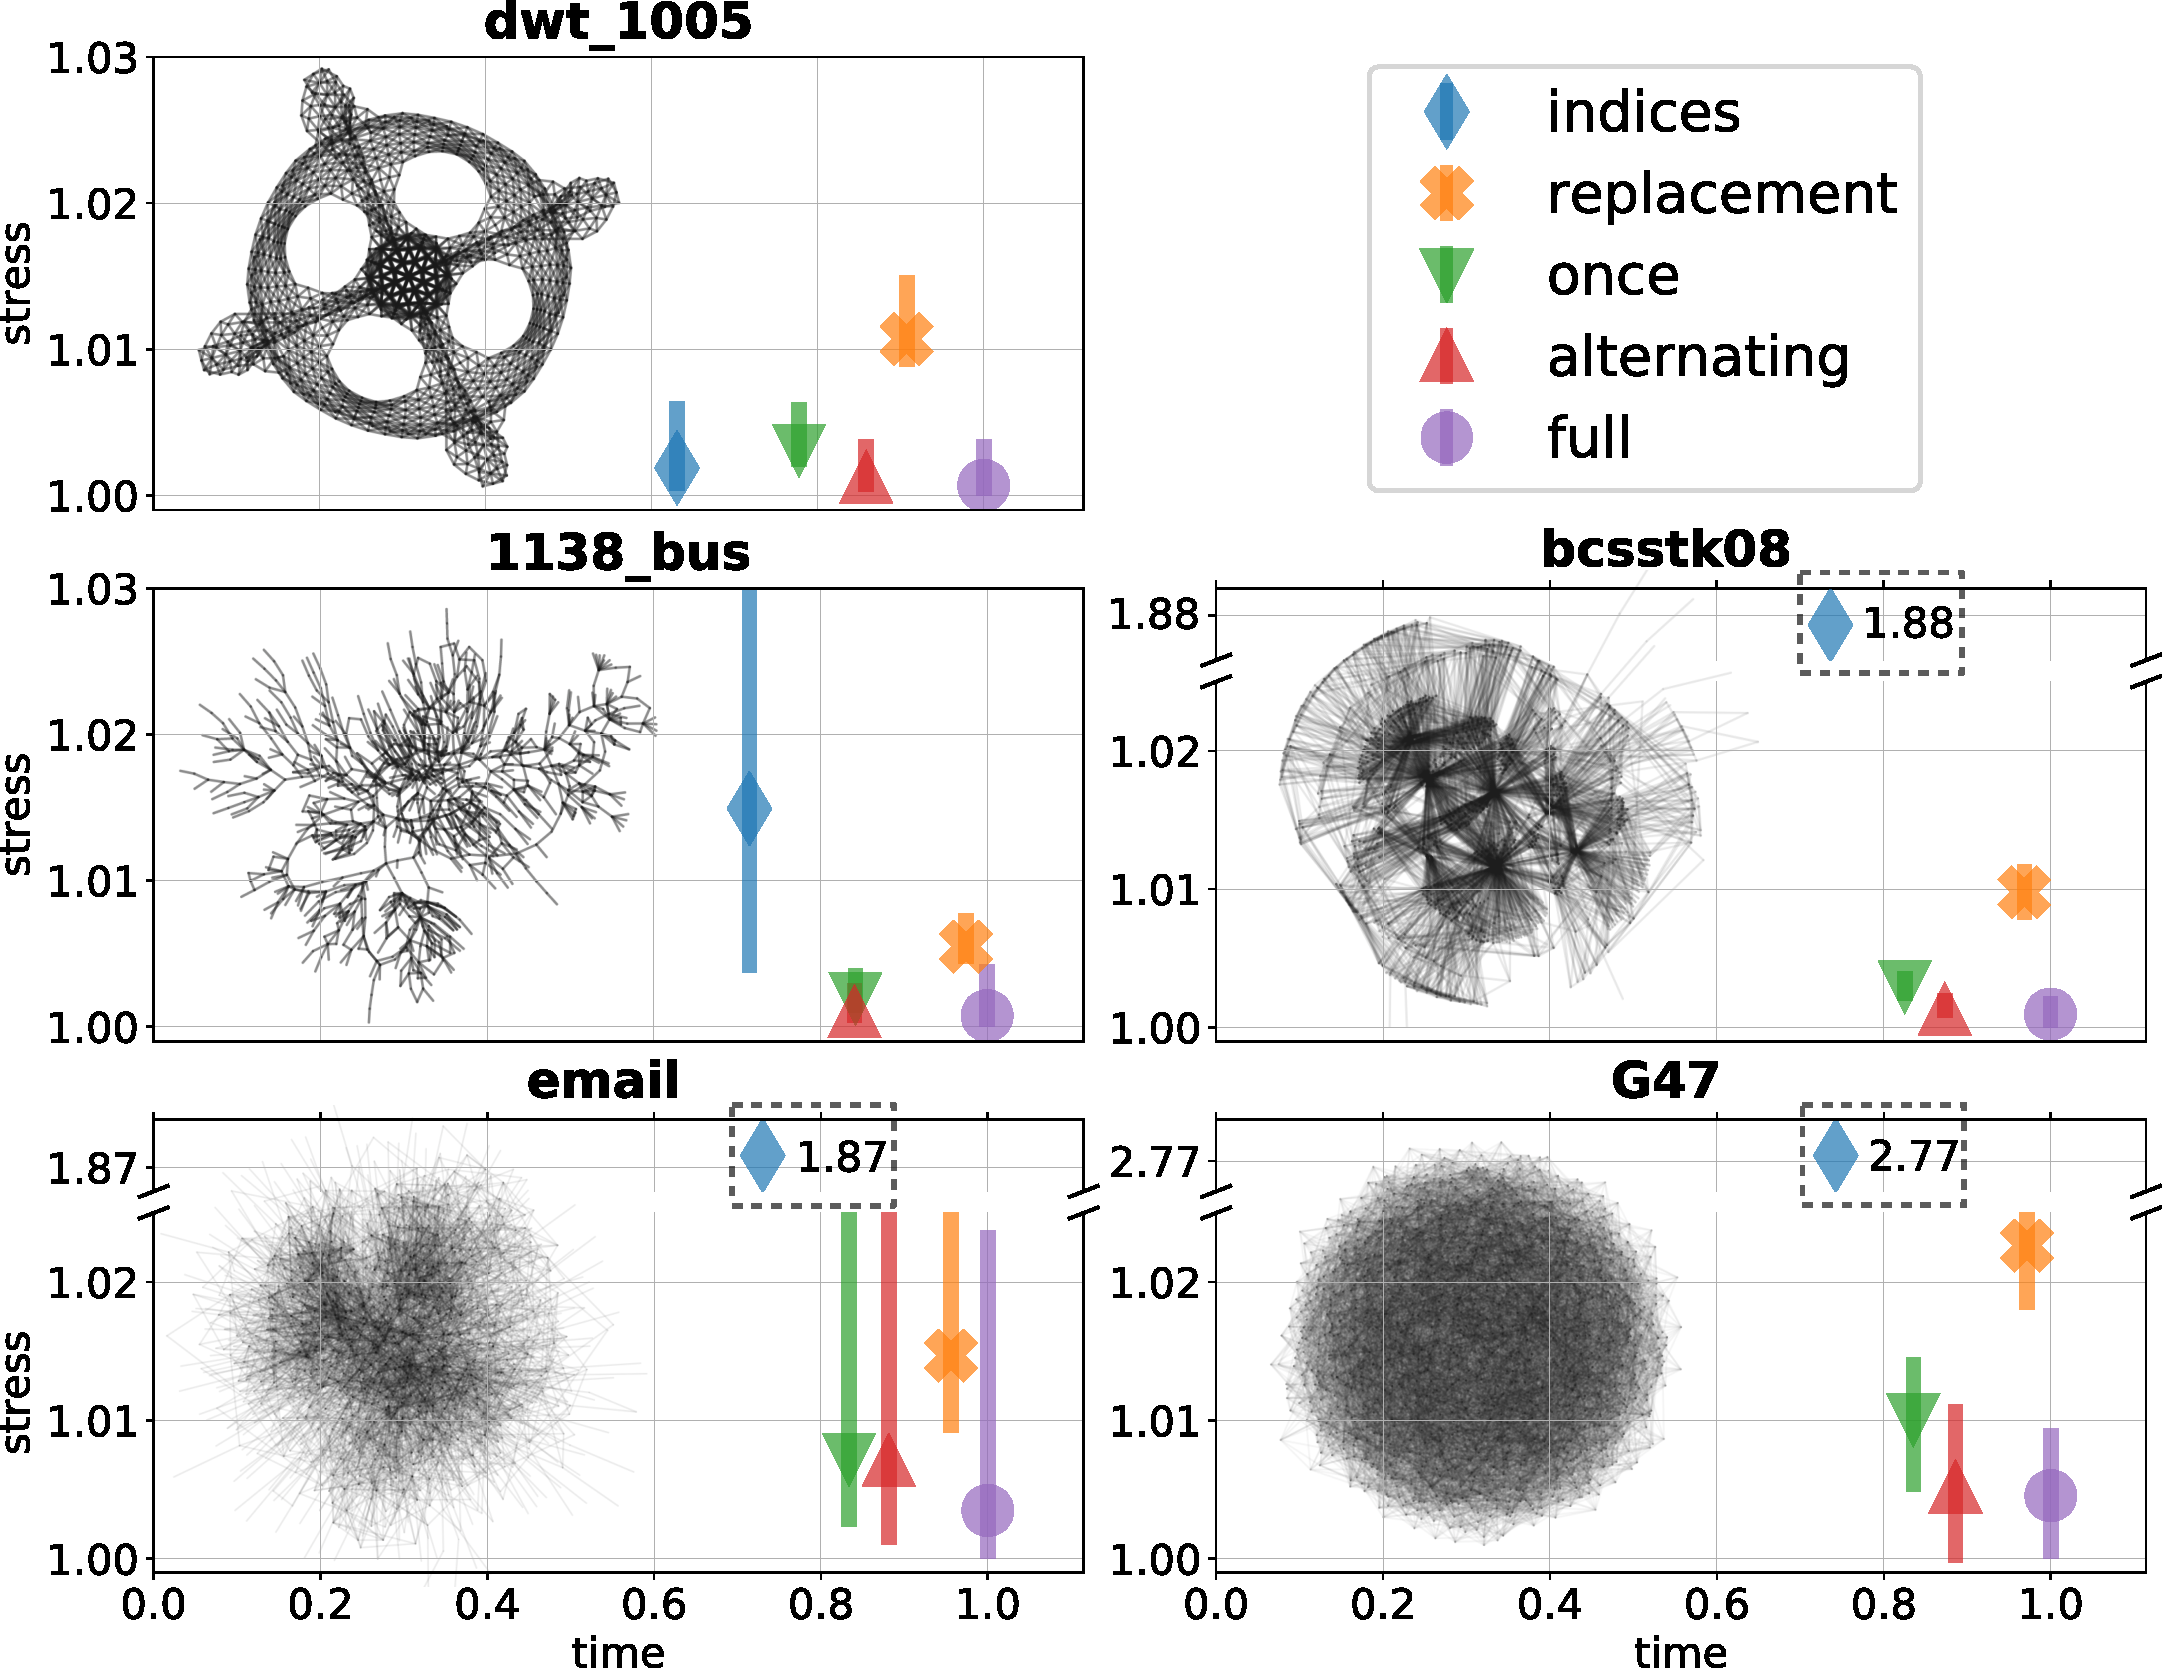
\includegraphics[width=.9\textwidth]{stress/random.pdf}
  \caption[A comparison of methods for term order randomisation]{Plots of stress against time, taken using different degrees of randomization, over 50 runs from different random starting configurations. Markers indicate mean stress, with vertical error bars ranging from best to worst over all runs.
  Graphs are arranged in order of mean stress, with both stress and time normalized to the absolute minimum and maximum respectively over any run.
  }
  \label{fig:randomisation}
\end{figure}

Unfortunately adding randomness incurs a penalty in speed, due to the cost of both random number generation and reduced data cache prefetching.
This overhead is non-trivial, with iterations taking up to 60\% longer with random reshuffling compared to looping in order. 
The trade-offs between more randomness for better convergence but slower iterations, versus less randomness for slower convergence but faster iterations, will therefore be explored here.
Five different degrees of randomness were tried: shuffling only the indices themselves, which removes any bias inherent to the data but still makes use of the cache by iterating in order; randomizing with replacement; shuffling the order of terms once; shuffling twice and alternating between the two orders; and shuffling on every iteration.
The results can be seen in Figure~\ref{fig:randomisation}.

Five different graphs were selected, each with around 1000 vertices, and show a corresponding good layout for each to visualize the differences between them.
More mesh-like graphs such as \texttt{dwt\_1005} do not benefit much from added randomness, and receive large gains in speed for a small hit to quality.
As graphs get more difficult to draw, shuffling only indices quickly becomes ineffective, with mean stress levels off by orders of magnitude on the plots with broken axes.
The graph \texttt{email} is a social network, which tend to be very difficult to draw as their global minima can be hard to find. The drop in quality when reducing the randomness reflects this. \texttt{G47} is a random graph and has the highest stress, but is easier to draw since there are many minima close to global that are all relatively easy to find. In other words, even a random layout would achieve a decent value for stress here.

Although RR is the most expensive method, it is only slightly more expensive and consistently performs best. However if speed is the most important concern, alternating between two random shuffles gives stress levels that are in many cases almost as good, at a slightly reduced cost.
RR is used for the rest of the results here.

\subsection{Systematic study}
\label{sec:sgd_experiment}
To test the effectiveness of SGD, symmetric sparse matrices from the SuiteSparse Matrix Collection \citep{Davis2011} will be used as a benchmark, following \citet{Khoury2012}.
Both SGD and majorization were ran on every graph with 1000 or fewer vertices, and compared the range of stress levels reached after 15 iterations and until convergence, using the two schedules described Section~\ref{sec:annealing}. These results can be seen in Figure~\ref{fig:systematic}.
Each graph in the collection is also assigned to a group as metadata, and graphs that share a group tend to have similar topologies; groups are kept together, ordered alphabetically, and within each group sorted by difference in mean stress when allowing for convergence. Thus both plots have the same order. Groups are demarcated by the alternating shaded background. 

A representative selection of larger graphs were also chosen for more detailed timing results, showing multiple implementations of majorization and the time course of convergence, which can be seen in Figure~\ref{fig:stress_plots_big}.

\begin{figure}
  \centering
  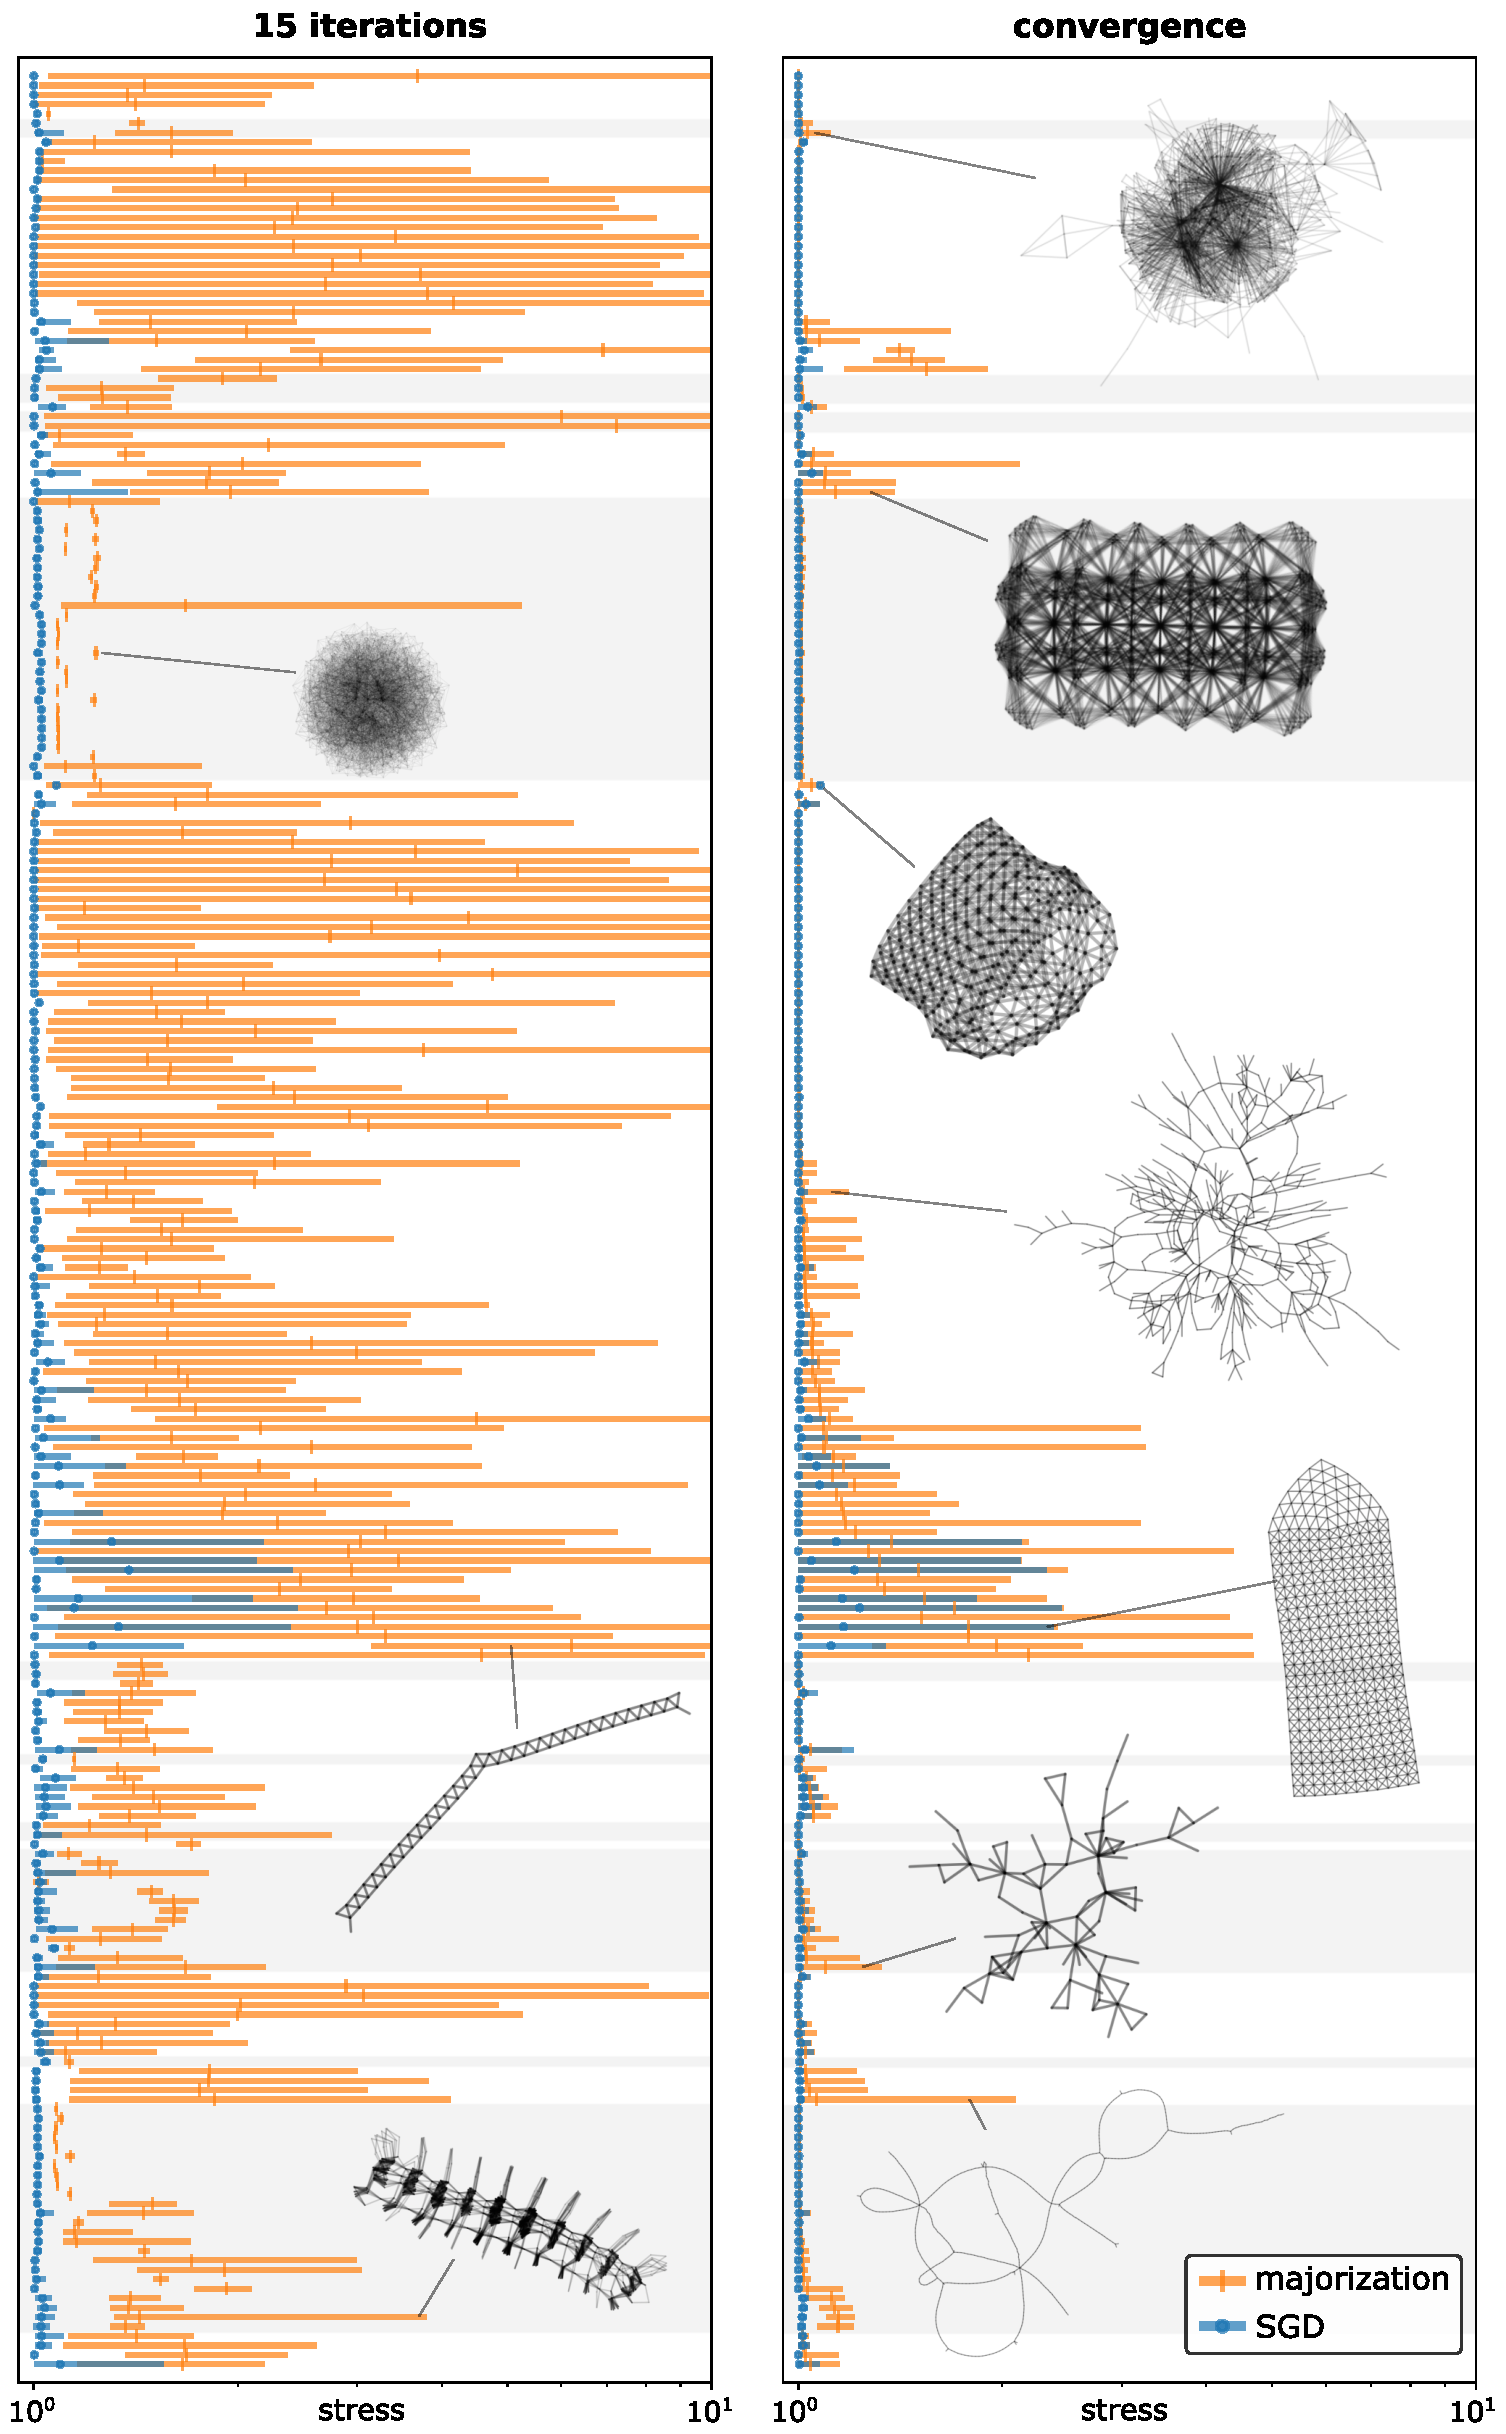
\includegraphics[height=.85\textheight]{stress/systematic.pdf}
  \caption[A systematic comparison against majorization over 243 graphs]{Stress achieved over 25 runs on 243 graphs in total. Markers indicate the mean over all runs, with bars ranging from minimum to maximum on any run.
  The left plot shows values reached after 15 iterations, and the right after convergence.
  Stress values are normalized to the lowest value achieved on all runs for either algorithm, as a baseline `correct' layout.
  Layouts shown are described in Section~\ref{sec:sgd_experiment}.
  An animated version of the left plot can be viewed at
%   \url{www.github.com/jxz12/stress\_systematic}.
  \url{www.youtube.com/watch?v=uv6Vw36KZ0k}.
  
%   Layouts shown are, from left to right, top then bottom:
%   \texttt{G15}, 
%   \texttt{dwt\_66}, 
%   \texttt{orbitRaising\_2}, 
%   \texttt{celegans\_metabolic},
%   \texttt{ex2},
%   \texttt{dwt\_307},
%   \texttt{494\_bus},
%   \texttt{dwt\_361},
%   \texttt{Sandi\_authors},
%   \texttt{S10PI\_n1}.
  }
  \label{fig:systematic}
\end{figure}

\begin{figure}
  \centering
  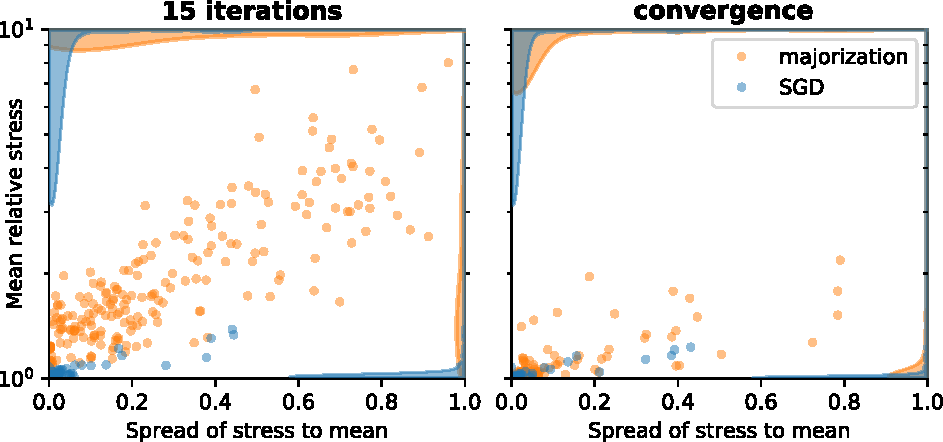
\includegraphics[width=.8\textwidth]{stress/systematic_summary.pdf}
  \caption[A summary of the results in Figure~\ref{fig:systematic}]{Scatter plots of mean stress relative to the best achieved, against the spread of the stress, measured as the coefficient of variation (standard deviation over mean), using the same results as Figure~\ref{fig:systematic}.
%     (left plot: 15 iterations, right plot: unlimited iterations).
%     Top plot is after 15 iterations and bottom is after 100. 
  The shaded regions on the top and right of each panel show the density of the mean (right) and spread (top) of the stress, computed using the \texttt{gaussian\_kde} function of SciPy \citep{Virtanen2020}.
  }
  \label{fig:systematic_summary}
\end{figure}

\subsubsection{Quality}
\label{quality}
Figure~\ref{fig:systematic} shows that that SGD reaches the same low stress levels on almost every run for both annealing schedules. While majorization is proven to monotonically decrease stress \citep{Gansner2004}, 
% this does mean that it cannot get stuck, and
it can often struggle with local minima. This can be clearly seen in Figure~\ref{fig:systematic_summary}, as majorization consistently shows larger variance in its stress trajectories from different starting configurations.

The layouts displayed in Figure~\ref{fig:systematic} were chosen to highlight the effects of different types of graphs. From left to right, top then bottom: \texttt{G15} is a random graph with nodes decreasing in mean degree. These random graphs reach consistent stress levels with both algorithms, as their lack of structure results in many minima close to global.
% They also take much more iterations to converge
\texttt{dwt\_66} is an example of a graph that majorization struggles with, as it is very long and often has multiple twists that majorization cannot unravel.
\texttt{orbitRaising\_2} is a similar example, but in this case majorization also never reaches the global minimum, even after convergence.
\texttt{celegans\_metabolic} is a metabolic pathway that is around as densely packed as a graph worth drawing gets.
SGD consistently outperforms majorization here too.
Many of the largest ranges in the plot are from graphs similar to \texttt{ex2}; grids are difficult to fully unfold, and majorization often struggles with their many local minima.

On the other hand, \texttt{dwt\_307} is the one graph (of the 243 investigated) where majorization reaches lower stress than SGD as a result of the modifications to standard SGD (see Figure~\ref{fig:cylinder}).

\begin{figure}
  \centering
  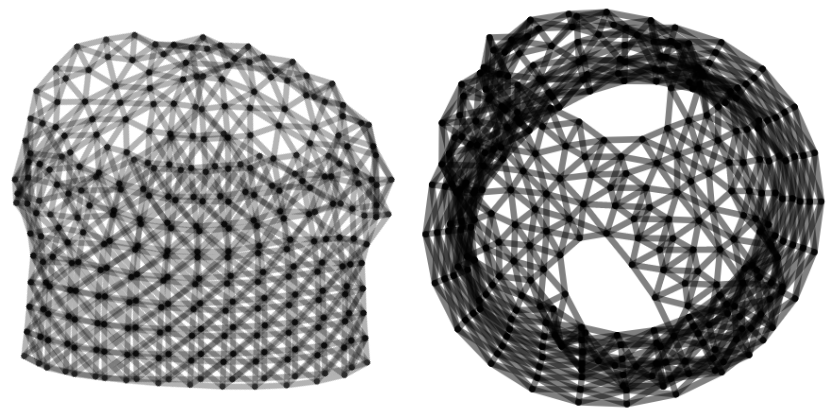
\includegraphics[width=1\textwidth]{stress/dwt_307.png}
  \caption[The one graph in the test set where majorization performs better]{Layouts from \texttt{dwt\_307}, the only one of the 243 graphs considered where majorization (left) yields lower stress than SGD (middle). The cylindrical shape of the graph is illustrated in a view of a 3D layout and projection on the right, which looks similar to if the middle layout were to be rotated slightly to the left.
  }
  \label{fig:cylinder}
\end{figure}

% \texttt{494\_bus} is an example of a very nice network to draw and is the type of graph where Equation~(\ref{stress}) shines. Its symmetry is clear here, whereas other force-directed algorithms can fail to show this due to the \emph{peripheral effect}~\citep{hu2005efficient}.
\texttt{494\_bus} is an example of the type of graph where stress as an energy function produces better layouts than other popular models. Its symmetry is clear here, whereas other force-directed algorithms can fail to show this due to the \emph{peripheral effect} \citep{Hu2005}.
\texttt{dwt\_361} is an example of the type of graph that both SGD and majorization struggle with: long graphs that can twist. A twist in a graph constitutes a deep local minimum that iterative methods struggle with in general, and SGD is still susceptible to this issue.
\texttt{Sandi\_authors} is a small graph, but with some densely packed sections that can become stuck behind each other, something that majorization often struggles with.
And finally, \texttt{S10PI\_n1} is a long graph that does not get twisted and so SGD deals with it perfectly well, but its long strands still tend to give majorization problems.

\subsubsection{Speed}
SGD converges to low stress levels in far fewer iterations than majorization. Graphs are laid out in only 15 iterations in the top plot in Figure~\ref{fig:systematic}, and there is not much improvement to be gained from using the convergent schedule to let the algorithm run for longer. This indicates that most global minima can be found in very few iterations, making SGD especially suited for real-time applications such as interactive layout.
The stopping criterion used for majorization was for relative decrease in stress to be less than $10^{\text{--}5}$, which is ten times more forgiving than originally suggested by \citet{Gansner2004}, as $10^{\text{--}4}$ was not lenient enough to be confident that it had settled completely. Given enough time, majorization does almost always eventually find good minima, but can still settle in suboptimal minima and in some cases never finds the best configuration regardless of initialization.
Majorization also takes many more iterations to converge than SGD, with means of 237 and 106 iterations respectively.

\begin{figure}
  \centering
  \makebox[\textwidth][c]{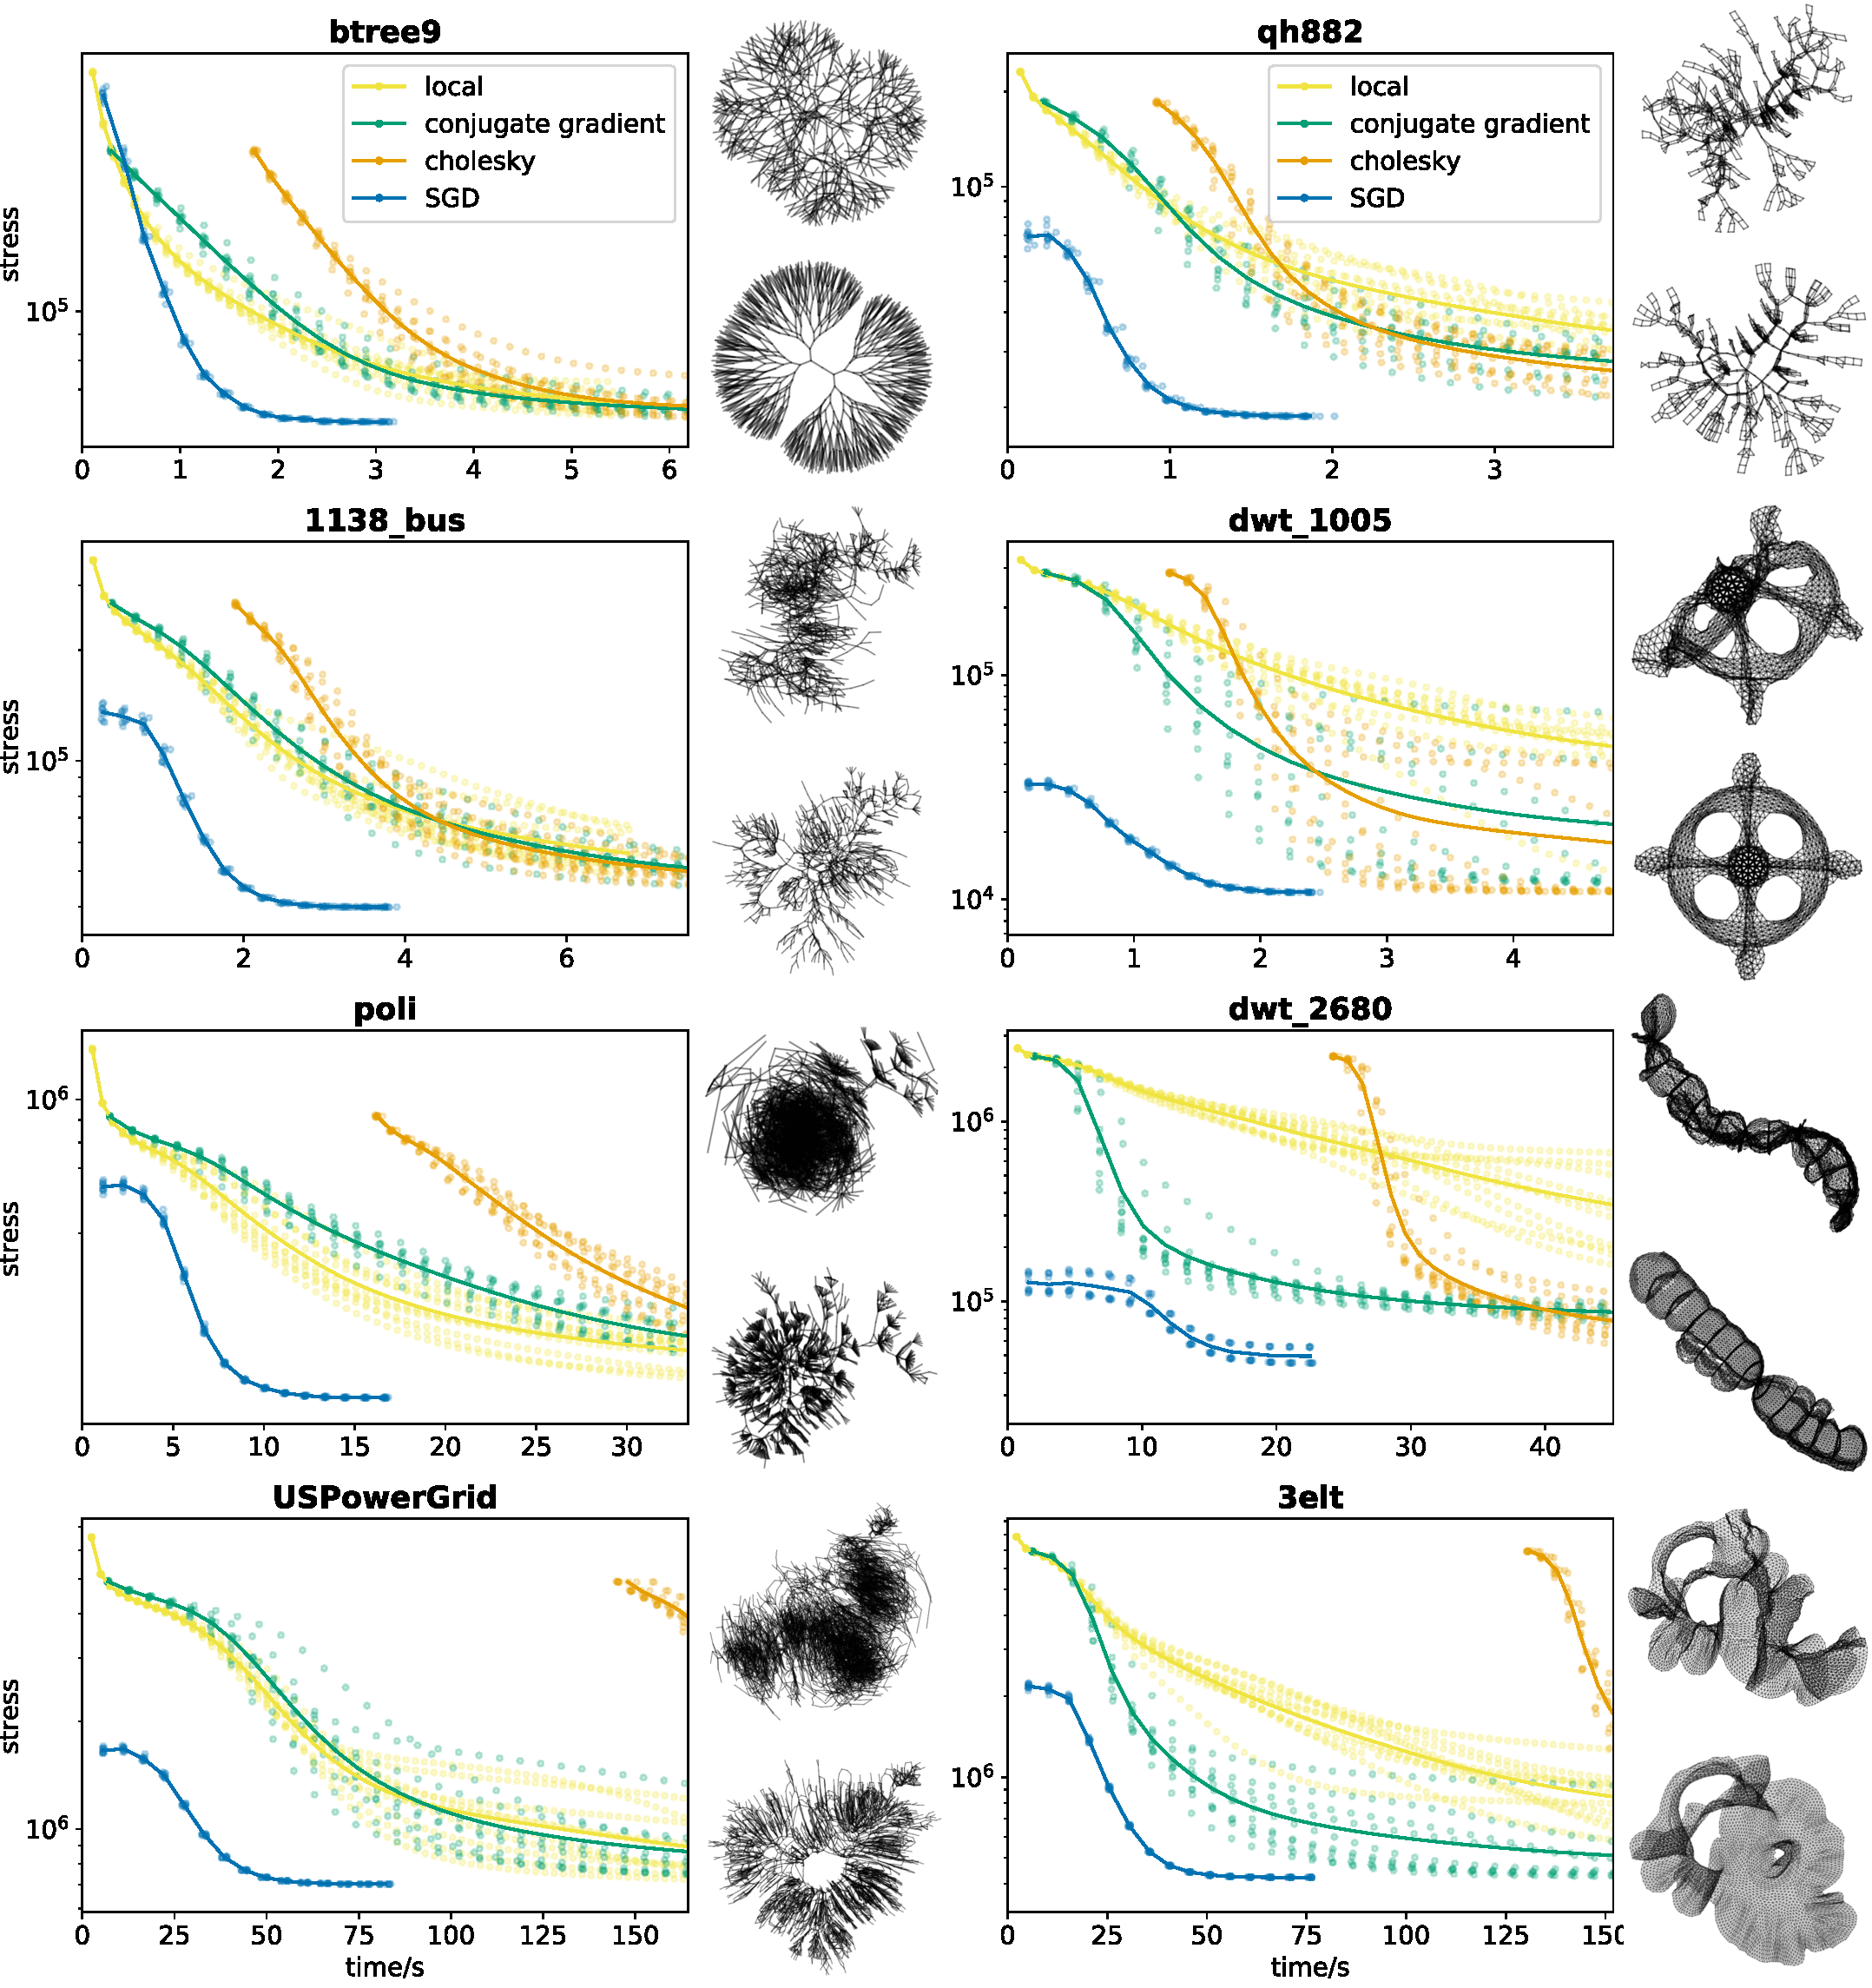
\includegraphics[width=1.09\textwidth]{stress/time.pdf}}
  \caption[Stress measured on a further selection of graphs]{Graphs of stress against time for all three implementations of majorization, and SGD using the 15 iteration annealing schedule. 10 runs were used for each method, and the line plots run through the mean stress and time per iteration.
  Graphs were considered as unweighted
  and layouts were initialized randomly within a 1$\times$1 square.
  The graph \texttt{btree9} is a binary tree of depth 9. 
  The layouts show examples of what the graphs look like after 15 iterations, with Cholesky on top and SGD on bottom.
  }
  \label{fig:stress_plots_big}
\end{figure}

The real-world time per iteration must also be considered, even though both share a complexity $O(|V|^2)$. The Cholesky factorization routine from Numerical Recipes \citep{Press2007Cholesky} was adapted to C\#, and found that iterations are around 40\% faster than SGD. However the initial decomposition before back-substitution requires $|V|^3/6$ iterations involving a multiply and a subtract \citep{Press2007Cholesky}, so the total time quickly tips in favor of SGD.
Conjugate gradient (CG), with tolerance 0.1 and max iterations 10 as in \citet{Gansner2013}, is an iterative method itself to solve the majorizing function and so iterates slower than Cholesky and SGD, but often beats out Cholesky overall when fewer iterations are necessary.
CG and Cholesky also both benefit from optimized matrix multiplication routines \citep{Gansner2004} that were not tried here.
Localized majorization, which is also used to for majorization in the sparse model to be studied in Section~\ref{sec:large_graphs}, iterates fastest of all but converges slowest.
It is also worth noting that over-shooting has been used before in the context of majorization to achieve an average of 1.5 times speedup \citep{Wang2012}.

Plots of stress against real time can be seen in Figure~\ref{fig:stress_plots_big}, where initial stress values are omitted, which is the cause of the horizontal offset to Cholesky due to its longer initialization time.
Note that if the time for the first iteration for Cholesky is removed, it outperforms the other implementations of majorization, but still does not ever drop below the curve for SGD.


\section{Large graphs}
\label{sec:large_graphs}
To understand how many layout algorithms tackle scaling to larger graphs, it is convenient to rewrite Equation~\eqref{eq:stress} by splitting the summation into two parts: paths that traverse one edge, and paths that traverse multiple.
This can be written as
\begin{equation}
  \text{stress}(\mathbf{X}) = \sum_{\{i,j\}\in E}w_{ij}\sigma_{ij}\\
  + \sum_{\{i,j\}\notin E}w_{ij}\sigma_{ij}
  \label{split stress}
\end{equation}
where $\sigma_{ij} = (||\mathbf{X}_i - \mathbf{X}_j|| - d_{ij})^2$.
Just considering the preprocessing stage for now, it is clear that $d$ and $w$ can be easily computed for the left half of the summation directly from the graph. Real-world graphs are also usually sparse, so for a graph with $|V|$ vertices and $|E|$ edges, $|E| \ll |V|^2$ making the space required to store these values tolerable. However the second half is not so easy --- an all-pairs shortest paths (APSP) calculation takes $O(|E| + |V|)$ time per vertex for an unweighted graph with a breadth-first search, or $O(|E| + |V|\log|V|)$ for a weighted graph using Dijkstra's algorithm \citep{Cormen2009}.

The second stage is iteration, where the layout is gradually improved towards a good minimum. Again, computing the first summation is tolerable, but the number of longer distance contributions quickly grows out of control. Many notable attempts have been made at tackling this second half. A common approach is to ignore $d_{ij}$, and to approximate the summation as an $n$-body repulsion problem, which can be efficiently well approximated using $k$-d trees \citep{Barnes1986}. \citet{Hu2005} and independently \citet{Hachul2004} used similar tricks in the context of the force-directed model of \citet{Fruchterman1991}, along with a multilevel coarsening scheme to avoid local minima. \citet{Gansner2013} use it with majorization by summing over $-\alpha \log||X_i - X_j||$ instead. \citet{Brandes2007Eigensolver} even ignore the second half completely and capture the long-range structure by first initializing with a fast approximation to \emph{classical scaling} known as PivotMDS \citep{Brandes2008}, which minimizes the inner product rather than Euclidean distance.

There are a couple of issues with this idea, one being that treating all long-range forces equally is unfaithful to
graph-theoretic distances,
and another being that the relative strength of these forces depends on an extra parameter that can greatly affect the final layout of the graph \citep{Hu2005}.
Keeping these dependent on their graph-theoretic distance sidesteps both of these issues, but brings back the problem of computing and storing shortest paths. One approach to maintaining this dependence comes from \citet{Khoury2012}, who use a low-rank approximation of the distance matrix based on its singular value decomposition. This can work extremely well, but still requires APSP unless $w_{ij} = d_{ij}^{-1}$.

\subsection{Sparse approximation}
\label{sec:sparse_explanation}
Within the normal MDS community, there have been multiple attempts to approximate stress, such as \citet{Halko2011} or GLINT \citep{Ingram2012}. However an additional problem with graphs is that shortest paths still need to be computed, and so even the distances between datapoints are not immediately available. This is an assumption that these approximations usually have, and so they cannot be directly used in the contexts of graphs.
% note that it does not really minimise a particular function because the weights are asymmetric.
Fortunately, \citet{Ortmann2017} developed an approach designed around graphs. They pick a set of `pivot' vertices whose shortest paths are used as an approximation for the shortest paths of vertices close to them.
Since this approach reduces the number of terms in the summation, using it in the context of SGD also reduces the amount of work per iteration.

To approximate the full model well it is important to choose pivots that are well distributed over the graph, and so \citet{Ortmann2017} presented an experimental evaluation of various methods for doing so. The implementation here uses \emph{max/min random sp} to select pivots. This was chosen because it gives good performance (second-best of all methods evaluated in terms of average reduction in stress) and the only method that performed slightly better, \emph{k-means sp}, is more complicated to implement and has a worse asymptotic complexity \citep{Ortmann2017}.

To further elaborate, ordinary (non-random) \emph{max/min sp} starts by picking one pivot randomly and computing its shortest paths to all other vertices, with subsequent pivots chosen by picking the vertex with the maximum shortest path to any pivot chosen so far \citep{DeSilva2004}. The random extension \emph{max/min random sp} instead samples for subsequent pivots with a probability proportional to shortest paths to any pivot, rather than simply always picking the maximum.
\emph{k-means sp} is also built upon \emph{max/min sp}, as it uses the calculated shortest paths as a high-dimensional embedding, exactly following the same first step as the layout method of \citet{Harel2004}. A standard $k$-means clustering algorithm is then applied to this embedding \citep{Friedman2001Nearest}, and pivots are chosen as the vertices closest the centroids of these clusters.
This extra clustering step is what pushes up the resulting asymptotic complexity \citep{Ortmann2017} which, in combination with the extra implementation work required, was why it was not chosen here.

These pivots $p\in P$ are then each assigned a region $R(p)$, which is the set of vertices closer to that pivot than any other. The relevant weights $w_{ip}$ are then adapted depending on the composition of the region, resulting in a new decomposed second half of the summation
\begin{equation}
  \begin{split}
  \text{stress}(\mathbf{X}) = \sum_{\{i,j\}\in E}w_{ij}\sigma_{ij}
  + \sum_{i\in V}\sum_{p\in P\setminus N(i)}w_{ip}'\sigma_{ij}
  \end{split}
  \label{eq:pivot_stress}
\end{equation}
where $N(i)$ are the neighbors of $i$ to prevent overlap with any edges in the first summation.
The adapted weight $w_{ip}'$ is then set to $s_{ip} w_{ip}$, where $s_{ip}$ is the number of vertices in $R(p)$ at least as close to $p$ as to $i$, defined as
\begin{equation}
  s_{ip}=|\{j\in R(p): d_{jp} \leq d_{ip}/2\}|.
  \label{eq:s}
\end{equation}
The reason the weight on vertex $i$ is increased like this is because its contribution acts as an approximation for the stress to all vertices in $R(p)$, and~\eqref{eq:s} is required to prevent the weight on closer vertices from being overestimated.
It is important to note that if both vertices $p$ and $q$ are pivots then $w_{pq}'$ may not equal $w_{qp}'$ and if only $p$ is a pivot then $w_{pq}'=0$ as $q$ should not contribute to the position of $p$.

This leaves far fewer terms in the summation, and so the complexity per iteration for SGD is now $\mathcal{O}(|E| + |P||V|)$, as any terms that have been cut are simply ignored. In the context of majorization this new model must be used with the local method described at the end of Section~\ref{sec:majorization}, resulting in the same complexity.

\begin{figure}
  \removeAlgorithmFigureError
  \begin{algorithm}[H]
    \SetKwProg{SGD}{SparseSGD}{}{} \SetKwInOut{Input}{inputs}
    \SetKwInOut{Output}{output}
    \SetKwFor{ForEach}{foreach}{:}{}
    \SetKwFor{For}{for}{:}{}
    \SetKwIF{If}{ElseIf}{Else}{if}{:}{elif}{else}{}
  
    \SGD{\emph{\textbf{(}}$G,h$\emph{\textbf{):}}}{
      \Input{graph $G=(V,E)$, number of pivots $h$}
      \Output{$k$-dimensional layout
      $\mathbf{X}$}
  
      $P \leftarrow \textsc{MaxMinRandomSP}(G,h)$
      \label{code:sparse:maxminrandom}
  
      $d_{pi} \leftarrow \textsc{SparseShortestPaths}(G,P)$
      \label{code:sparse:sparseshortestpaths}
      
      $w_{pi}' \leftarrow 0$
  
      \ForEach{$\{p,i\}\in (P \times V) : p \notin N(i)$}{
        $s \leftarrow |\{j\in R(p): d_{pj} \leq d_{pi}/2\}|$
  
        $w_{ip}' \leftarrow s \, w_{ip}$
        \label{code:sparse:sparse:s}
      }
  
      \ForEach{$\{i,j\} \in E$}{
        $w_{ij}' \leftarrow w_{ji}' \leftarrow w_{ij}$
      }
  
      $\mathbf{X} \leftarrow \textsc{Rand}(|V|,k)$
  
      \For{$\eta$ \emph{in $\textsc{AnnealingSchedule}()$}}{
        \ForEach{$\{i,j\} \in E \cup (P \times V)$ \emph{in random order}}{
  
          $\mu_i \leftarrow Min(w_{ij}' \eta \,,\ 1)$
  
          $\mu_j \leftarrow Min(w_{ji}' \eta \,,\ 1)$
  
          $\mathbf{r} \leftarrow \frac{||\mathbf{X}_i - \mathbf{X}_j|| - d_{ij}}{2}\frac{\mathbf{X}_i - \mathbf{X}_j}{||\mathbf{X}_i - \mathbf{X}_j||}$
  
          $\mathbf{X}_i \leftarrow \mathbf{X}_i - \mu_i \mathbf{r}$
  
          $\mathbf{X}_j \leftarrow \mathbf{X}_j + \mu_j \mathbf{r}$
        }
      }
    }
    \caption{Sparse SGD}
    \label{alg:sparse}
  \end{algorithm}

  \caption[Pseudocode for sparse stochastic gradient descent]{Pseudocode for performing SGD on the sparse stress approximation described in Section~\ref{sec:sparse_explanation}.
  Note that all $R(p)$ and $w_{ip}'$ can be constructed over the course of shortest path calculations without increasing the asymptotic complexity \citep{Ortmann2017} by using a multi-source shortest paths algorithm.
  \label{fig:pseudo_sparse}
  }
\end{figure}

\begin{figure}
  \centering
  \makebox[\textwidth][c]{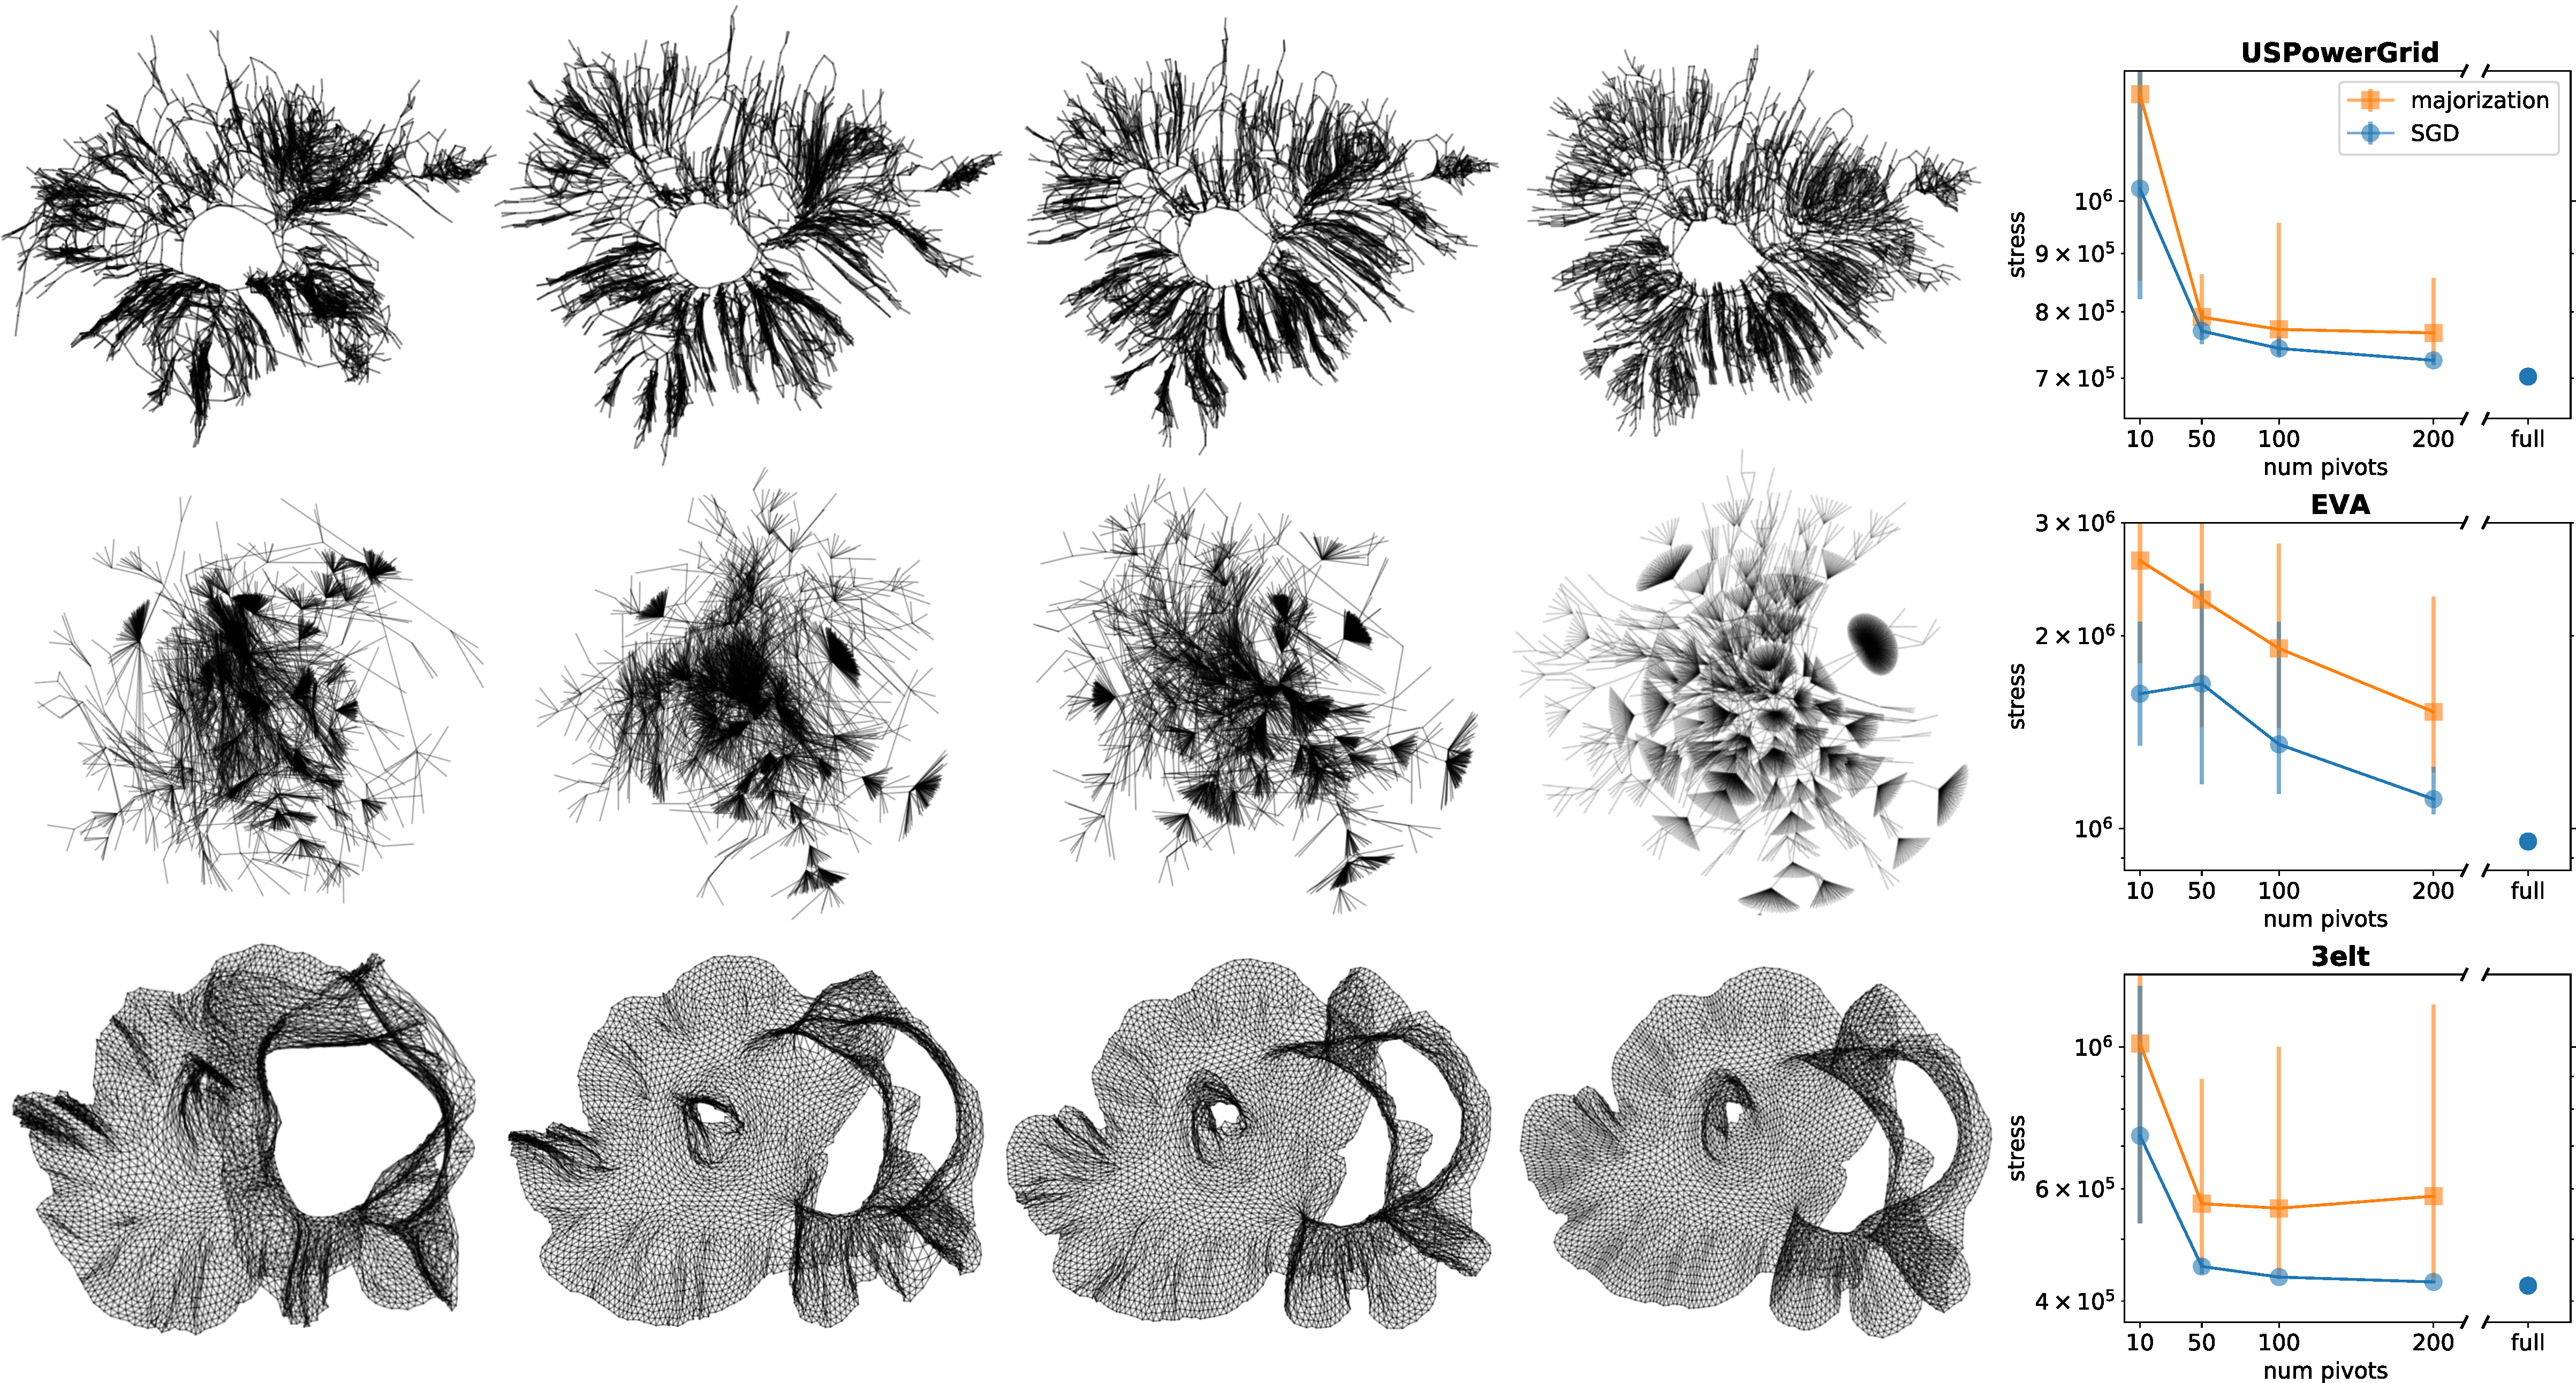
\includegraphics[width=1.06\textwidth]{stress/ortmann.pdf}}
  \caption[Results against majorization using sparse stress]{Examples of sparse SGD on the graphs \texttt{USPowerGrid}, \texttt{EVA}, and \texttt{3elt}. From left to right: best layouts using 10 pivots, 50, 200, full stress, and plots showing stress over 25 runs for each number of pivots.
  The 15 iteration annealing schedule from Section~\ref{sec:annealing} is used for SGD, and majorization is allowed to run for 100 iterations.
  }
  \label{fig:pivots}
% \end{figure}
  \vspace*{\floatsep}
% \begin{figure}
  \centering
  \makebox[\textwidth][c]{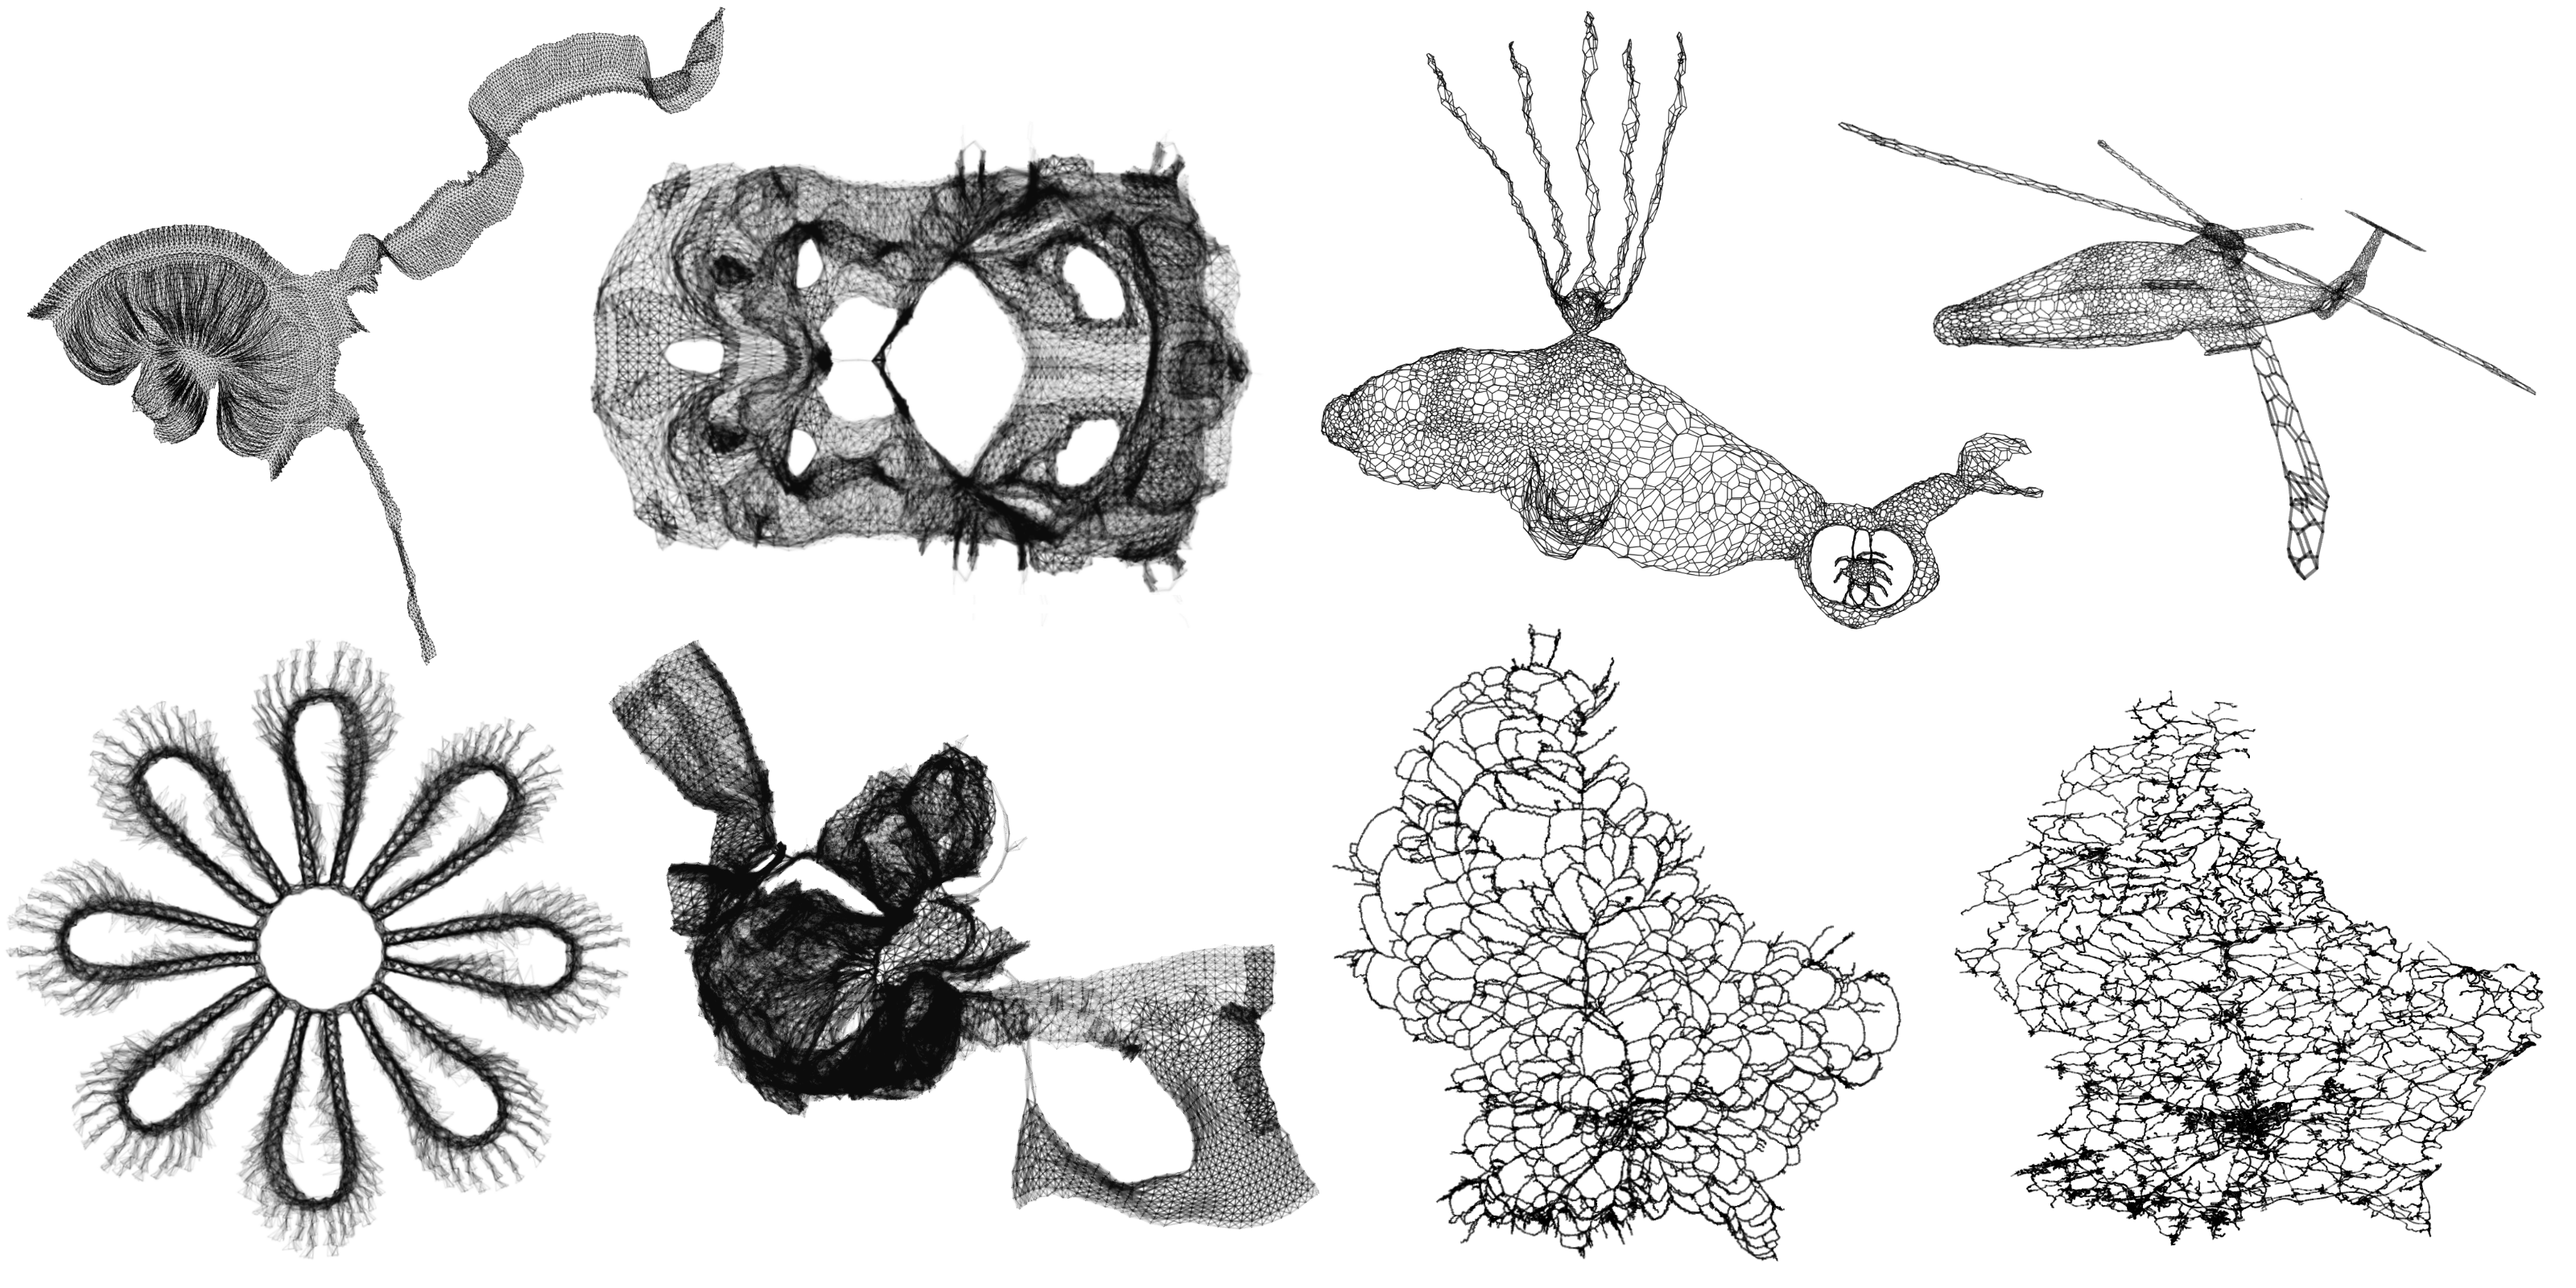
\includegraphics[width=1.02\textwidth]{stress/showcase.png}}
  \caption[A gallery of large graphs layed out using sparse stress]{Some larger graphs, each approximated with 200 pivots.
  %, also using the 15 iteration schedule from Section~\ref{sec:annealing}.
  From left to right, top row then bottom: \texttt{pesa} (11,738 vertices), \texttt{bcsstk31} (35,588), \texttt{commanche\_dual} (7,920) and its original (3D) layout, \texttt{finance256} (37,376), \texttt{bcsstk32} (44,609), \texttt{luxembourg\_osm} (114,599) and its original layout. The right-hand graphs have edge weights calculated from distances in their original layouts.
  }
  \label{fig:showcase}
\end{figure}

Resulting layouts are presented in Figures~\ref{fig:pivots}, where the graph \texttt{EVA} is the least well approximated by the sparse model, likely due to its low diameter and high degree distribution. \texttt{3elt} is very well approximated by the model itself, but the performance of majorization declines as the number of pivots exceeds ${\sim}100$, likely due to the increased number of terms in the summation that introduce more local minima to jump over.
Note that the results here do not use PivotMDS \citep{Brandes2007Eigensolver} to initialize as done by \citet{Ortmann2017}, and instead initialize randomly within a 1$\times$1 square as before.
A gallery of larger graphs is presented in and~\ref{fig:showcase}, and pseudocode for the entire algorithm can be seen in Algorithm~\ref{alg:sparse}, Figure~\ref{fig:pseudo_sparse}.


\section{Applications}
\label{sec:cookbook}
A benefit of force-directed algorithms is the possibility of making ad hoc changes to the optimisation process, to change the visualisation in a domain-specific manner. For example, nails can be used to hold a node in place \citep{Mi2016}, magnetic fields can be used to align nodes in various ways \citep{Sugiyama1994}, and complex attractive and repulsive forces can be used to highlight clusters \citep{Suh2019}.

Some of the properties of SGD, in particular the fact that each edge is considered separately along with the ability to consistently avoid local minima well, make SGD well suited to such additional modifications. This section will describe some recipes for examples of this, each applied to various real-world graphs in order to show the merits of their use.
Note that these applications are also possible with majorization, but can require more drastic modifications in order to apply them successfully.

\subsection{Radial layout}
\label{sec:sgd_radial}

It is often the case that a user will want to examine specific vertices in a graph, especially in an interactive setting. It is therefore important to be able to emphasize distances involving certain vertices.
\citet{Brandes2011} presented a general method of doing this in the context of majorization, by interpolating between two stress summations representing general and constrained weights separately.

For SGD, emphasizing specific distances is as simple as weighting the corresponding constraints more heavily.
For example to focus on vertex 3, the relevant weights are set to infinity
\begin{equation}
  w_{ij} \leftarrow \infty \quad \text{if}\ i=3\ \text{or}\ j=3.
\end{equation}
This causes only the remaining constraints to decay, but the system still converges in this case as there are no conflicts between the ones emphasized. Exploding gradients are still prevented by the capping of the step size in Equation~\eqref{eq:mu}.
An important remaining step is that the step size must be allowed to decay for extra iterations, in order to allow the infinitely weighted terms to essentially become the only remaining contribution at convergence. 
An example of this method in action can be seen in Figure~\ref{fig:tube}.\footnote{Data collected from
\url{www.github.com/petertrotman/london-underground-travel-time-map}, accessed 13/8/20.}

\begin{figure}
  \centering
  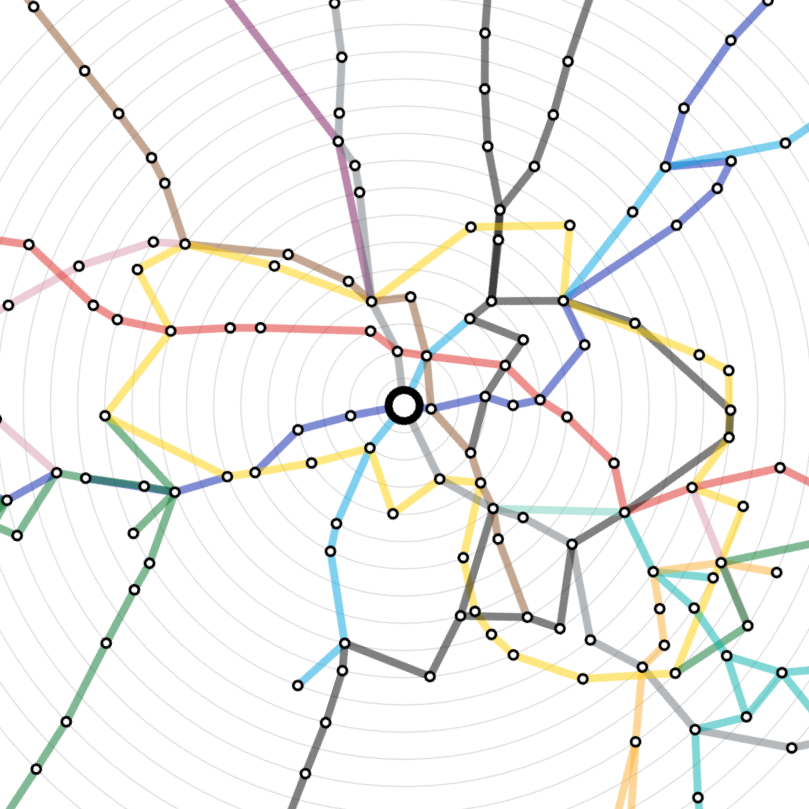
\includegraphics[width=0.7\textwidth]{stress/tube.png}
  \caption[The London tube map with a focus on Green Park station]{The London Underground map with a focus on Green Park, created using the method described in Section~\ref{sec:sgd_radial}. The distances are based on travel time rather than real world distance.}
  \label{fig:tube}
\end{figure}

Setting weights to infinity when using majorization results in the algorithm becoming instantly very stuck, which is why the more complicated interpolation \citep{Brandes2011} is necessary.

This idea of editing individual constraints can also be used to pin nodes in place. This could be done by not allowing pinned nodes to be moved when satisfying the constraint as in Figure~\ref{fig:satisfaction}. Additionally if many nodes are pinned, then any constraints between pinned nodes can be left out of the objective function entirely, reducing the amount of computation time required.


\subsection{General multidimensional scaling}
\label{sec:normal_mds}
Stress as an energy function originated as a general visualisation algorithm for embedding high-dimensional data, and using SGD to optimize it does not change its ability to perform this original function. Here this will be shown by applying it on a distance measure other than the graph-theoretic shortest path, in order to show its versatility. The measure that will be used is the Jaccard index, which can be defined as a distance by
\begin{equation}
  d_{ij} = 1 - \frac{|N(i) \cap N(j)|}{|N(i) \cup N(j)|}
  \label{eq:jaccard_sgd}
\end{equation}
where $N(i)$ is the set of neighbors of vertex $i$. This is effectively a measure of how similar the neighbour sets of vertices $i$ and $j$ are to each other.
This measure will be applied on top of an existing graph layout, but since the two spacial dimensions are already being used, the three-dimensional space of \emph{colour} will be used instead.

\begin{figure}
  \centering
  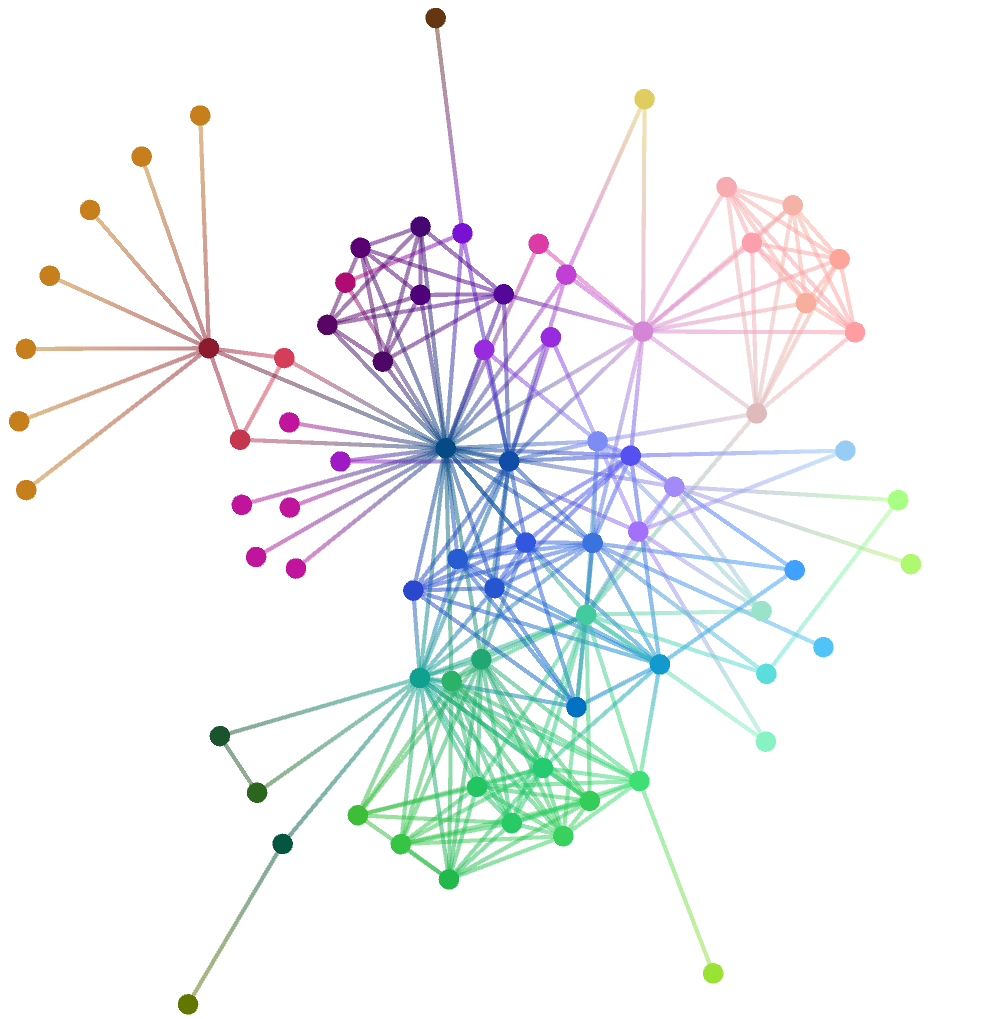
\includegraphics[width=.7\textwidth]{stress/lesmis.png}
  \caption[A graph \texttt{lesmis} with node colours embedded in RGB space]{
  Co-appearances of characters in Les Mis\'erables by Victor Hugo \citep{Knuth1993}.
  Groups of similarly colored vertices indicate clusters based on Jaccard dissimilarity as in Equation~\eqref{eq:jaccard_sgd}.
  }
  \label{fig:jaccard}
\end{figure}

Since color is simply a linear mix of red, green, and blue (RGB), it can be used as a 3D space in which Euclidean distances can be embedded, where each color corresponds to a separate axis. Ideally a perceptually uniform colour space would be used such as CIELAB \citep{Smart2019}, but in this small illustrative example it was not necessary.
Since the Jaccard distance is bounded between $0\leq d_{ij}\leq 1$, embedded distances fit perfectly within the similarly bounded axes of color. This means that vertices not only have coordinates within normal Euclidean space, but also within RGB space. 
An illustration of this can be seen in Figure~\ref{fig:jaccard}, where vertices are coloured according to their (secondary) embedding in RGB space. Note that in this case $w_{ij}$ is simply set to one.

This process can help to reveal groupings, but can also produce ambiguity when applied to larger graphs due to the lack of distinct color combinations, again a problem caused by a lack of output dimensions. One possibility in this case would be to use an interactive form of visualization in which the user selects a smaller group of vertices at a time, and the algorithm embeds only their selection in an RGB space, by considering dissimilarities only between selected vertices.

\section{Discussion}
One of the major reasons why previous force-directed algorithms \citep{Eades1984,Kamada1989,Fruchterman1991,Frick1995},
have become popular is how simple and intuitive the concept is. The idea of a physical system pushing and pulling vertices, modeled as sets of springs and electrical forces, makes them easy to understand and quick to implement for practical use.

The geometric interpretation of the SGD algorithm presented here shares these qualities, as the concept of moving pairs of vertices one by one towards an ideal distance is just as simple.
In fact the stress energy function in Equation~\eqref{eq:stress} is commonly known as the \emph{spring model} \citep{Kamada1989,Hu2005}, and so the physical analogy of SGD to decompressing one spring at a time very naturally fits this intuition.
The implementation also requires no equation solver, and there is no need to consider smart initialization, which can often be just as complex a task \citep{Brandes2008}.
Considering only a single pair of vertices at a time also makes further constrained layouts easy to implement, and allows an appropriate sparse approximation to grant scalability up to large graphs.

But perhaps the most important benefit of SGD is its consistency regardless of initialization, despite being non-deterministic due to the shuffling of the order of terms. By contrast, the plots in Section~\ref{sec:sgd_experiment} clearly show how vastly the results from majorization can differ depending on initialization, especially when restricted to a limited number of iterations. This reliability of SGD can be crucial for real-time applications with fixed limits on computation time, such as within an interactive visualization.

However there are still situations where SGD can struggle with local minima, such as \texttt{dwt\_2680} which is susceptible to twisting in the middle. This can be seen in Figure~\ref{fig:stress_plots_big} where a twisted layout is purposefully included to illustrate this pitfall.
A potential solution to this is overshooting, or in other words allowing values of $0 < \mu < 2$ in Equation~\eqref{eq:mu}. This greatly reduces the chance of a twist, but results in poorer local minima in most other cases and can also bring back the problem of divergence, so is a potential avenue for future work,
perhaps to be used in conjunction with an adaptive annealing schedule to further optimize performance depending on the input data.

Another valid option is to set the maximum value of $\mu$ to a value somewhere in between one and two. This will be used in Chapter~\ref{chap:joy}, Section~\ref{sec:eco_visualisation} for a real-world application, where it will be shown that allowing a slightly higher maxiumum step size is in fact necessary for another domain-specific application, on top of the ones shown in Section~\ref{sec:cookbook}.

Interaction could also allow the user to manually adjust the step size $\eta$ from Equation~\eqref{eq:SGD_step}, allowing them to `shake' the graph out of local minima themselves. The step size annealing from Section~\ref{sec:annealing} is the most ad hoc and data-dependent component of SGD, so handing control over to the user could help, especially in dynamical situations where the structure of the graph changes with time.
Additionally, if frame rate becomes an issue in an interactive setting, the application does not have to wait until the end of an entire iteration before rendering an updated layout, because vertices are continually being moved at each satisfaction step. This would keep the application smooth and responsive, whilst still giving an indication of the algorithm's progress.

\subsubsection{Conclusion}
This chapter has presented a modified version of stochastic gradient descent (SGD) to minimize stress as defined by Equation~\eqref{eq:stress}. An investigation comparing the method to majorization shows consistently faster convergence to lower stress levels, and the fact that only a single pair of vertices is considered at a time makes it well suited for variants such as domain-specific modifications or the pivot-based approximation of \citet{Ortmann2017}.
This improved performance --- combined with a simplicity that forgoes an equation solver or smart initialization --- makes
SGD a strong candidate for general graph layout applications.

All code used for timing experiments, along with a fast C++ implementation with a Python wrapper, is open source and available at \url{www.github.com/jxz12/s_gd2}.%\footnote{The name \texttt{s_gd2} stands for $s(gd)^2$, with letters corresponding to the name of the paper in \citep{Zheng2019Stochastic}. Unfortunately, a better name is...}